
\chapter{\'Etude du corpus d'évaluation \textit{ambiance}}
\label{chap:ambiance}
Dans ce chapitre, on étudie le comportement des différentes versions de la NMF, présentées dans le chapitre \ref{chap:nmf},  avec le premier corpus élémentaire \textit{Ambiance}. 
Dans un premier temps un rappel du corpus, des méthodes choisies et une présentation de la méthode de référence (ou \textit{baseline} en anglais) sont présentés. Puis les étapes menant à l'apprentissage du dictionnaire et l'ensemble des facteurs expérimentaux sont détaillées. Enfin les résultats des calculs menés sont présentés et discutés.


\section{Rappel de la méthode employée}

Les étapes impliquées dans l'estimation du niveau sonore du trafic à partir de scènes sonores simulées sont d'abord rappelées. La Figure \ref{fig:rappel_estimateur} résume la démarche générale.

\begin{figure}[ht]
\centering
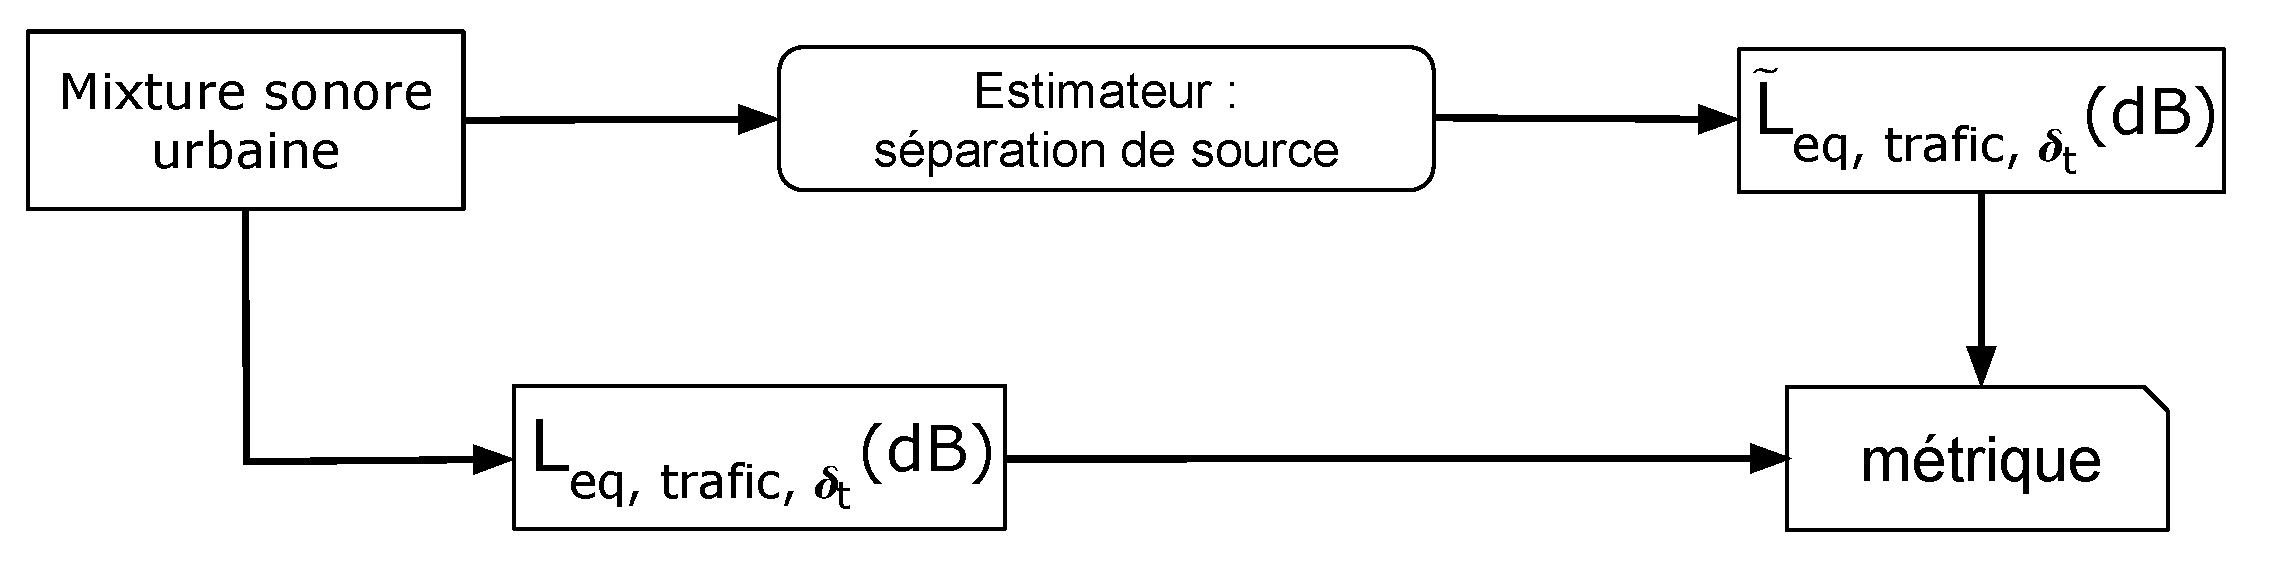
\includegraphics[width=.8\linewidth]{./figures/NMF/Bloc_diagram_estimateur_FR.pdf}
\caption{Diagramme en blocs dans l'estimation du niveau sonore du bruit de trafic}
\label{fig:rappel_estimateur}
\end{figure}

Le corpus de scènes sonores a été présenté dans \ref{part:corpus_ambiance} et est composé, pour rappel, de 6 sous-corpus : \textit{alerte}, \textit{animaux}, \textit{climat}, \textit{humain}, \textit{transport}, \textit{mécanique}. Chaque sous-corpus est lui-même divisé en 5 sous-ensembles qui comprennent 25 mixtures sonores de 30 secondes, comprenant une classe de son \textit{trafic} (qui inclut le bruit de fond routier ainsi que les évènements sonores \textit{passages de voitures}), $S_{tr.}$, et une classe de son \textit{interférante} (qui regroupe tous les autres sources sonores), $S_{int.}$ : 

\begin{equation}
M_i = S_{tr.,i}+S_{int.,i}.
\end{equation}

Dans chaque sous-ensemble, le niveau sonore du signal \textit{trafic}, $L_{eq,trafic}$ est calibré par rapport au niveau sonore de la classe de son \textit{interférante}, $L_{eq,interferant}$ tel que : 

\begin{equation}
TIR = L_{eq,trafic} - L_{eq,interferant}
\end{equation}

avec $TIR \in \lbrace -12,~-6,~0,~6,~12 \rbrace$. Ce corpus permet de tester les performances de la NMF et son comportement face à différentes sources sonores avec une prédominance variable du trafic routier. En tout, le corpus est composé de 750 scènes pour une durée totale de 6h30.

Pour chaque TIR et chaque sous-corpus, les 25 scènes sont soumis à un estimateur qui détermine le niveau sonore de l'intégralité de la scène en dB \textit{trafic},  $\tilde{L}_{eq,trafic, i}$. Les 25 niveaux sonores sont ensuite comparés à leurs niveaux sonores exactes respectifs, $L_{eq,trafic, i}$ au travers de la métrique $MAE$ (équation \ref{eq:mae} définie dans la partie \ref{part:cachier_charges}). Il est ensuite possible de déterminer les performances d'un estimateur sur l'ensemble des 6 sous-corpus pour chaque TIR en calculant sa moyenne :

\begin{equation}
MAE_{TIR} = \frac{\sum_{i = 1}^6 MAE_{i}}{6}.
\end{equation}

Il est enfin possible de calculer une erreur global sur l'intégralité du corpus \textit{Ambiance} pour connaitre l'estimateur qui permet, quelque soit le TIR ou le sous-corpus, l'erreur moyenne la plus faible : 

\begin{equation}
MAE_{globale} = \frac{\sum_{i = 1}^6 \sum_{j = 1}^5 MAE_{i,j}}{6 \times 5}.
\end{equation}

C'est cet indicateur traduit l'erreur moyenne de l'estimateur sur l'ensemble des cas et ainsi l'erreur qui serait faite si aucune connaissance \textit{a priori} sur l'environnement sonore est disponible.

\section{Estimateur baseline}
Dans un premier temps, un estimateur de référence (ou \textit{baseline} en anglais) est nécessaire afin de comparer les performances de la NMF. La baseline choisie est un filtre en fréquence passe-bas de fréquence de coupure $f_c$. L'hypothèse faite est qu'en rejetant l'énergie au delà de $f_c$, l'énergie conservée est assimilable au signal \textit{trafic}, $\tilde{L}_{eq,trafic}$. Ce choix est justifié par la présence de composantes basses-fréquence (< 1000 Hz) dans les signaux trafic. De plus, cet outil, aussi simple soit-il, est celui qui aurait pu être choisi par défaut.
Cet estimateur consiste à représenter une mixture $M_i$ sous la forme d'un spectrogramme puis à rejeter toutes les trames fréquentielles supérieurs à $f_c$. La Figure \ref{fig:baseline} résume les étapes intervenant pour cet estimateur.

\begin{figure}[hbtp]
\centering
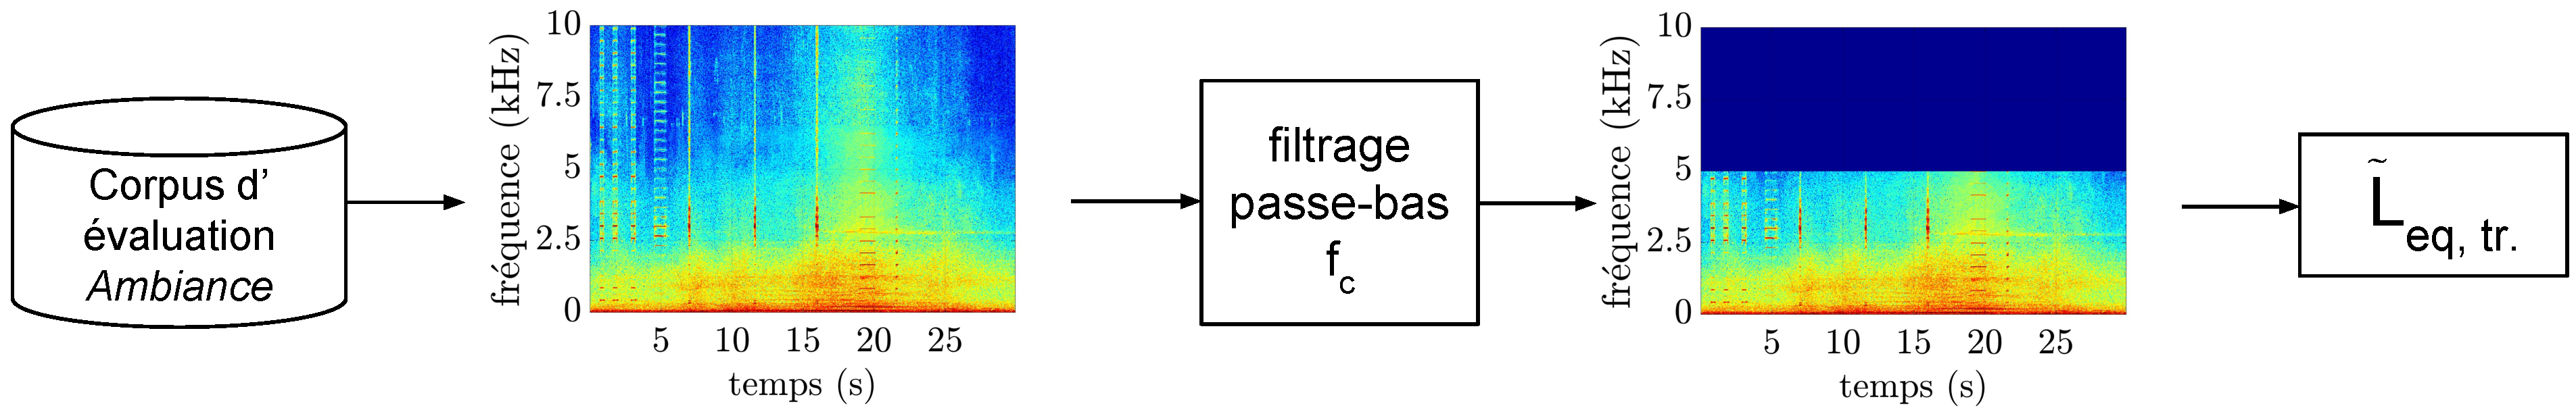
\includegraphics[width=\linewidth]{./figures/NMF/filtre_principe.pdf}
\caption{Principe de l'estimateur \textit{baseline}  pour une mixture sonore filtrée à $f_c$ = 5kHz.}
\label{fig:baseline}
\end{figure}

Les fréquences de coupures choisies sont alors $f_c = \lbrace 100, 500, 1k, 2k, 5k, 10k, 20k \rbrace$ Hz. Le cas où $f_c = 20$ kHz correspond finalement au cas où aucun traitement du signal n'est réalisé sur les fichiers audio et où toutes les sources présentes sont assimilées au trafic.

\section{Estimateur basé sur la NMF}
Le second estimateur est celui basé sur la NMF, présentée dans le chapitre \ref{chap:nmf}. La Figure \ref{fig:nmf_ambiance} rappelle les différentes étapes présentes dans cet estimateur.

\begin{figure}[ht]
\centering
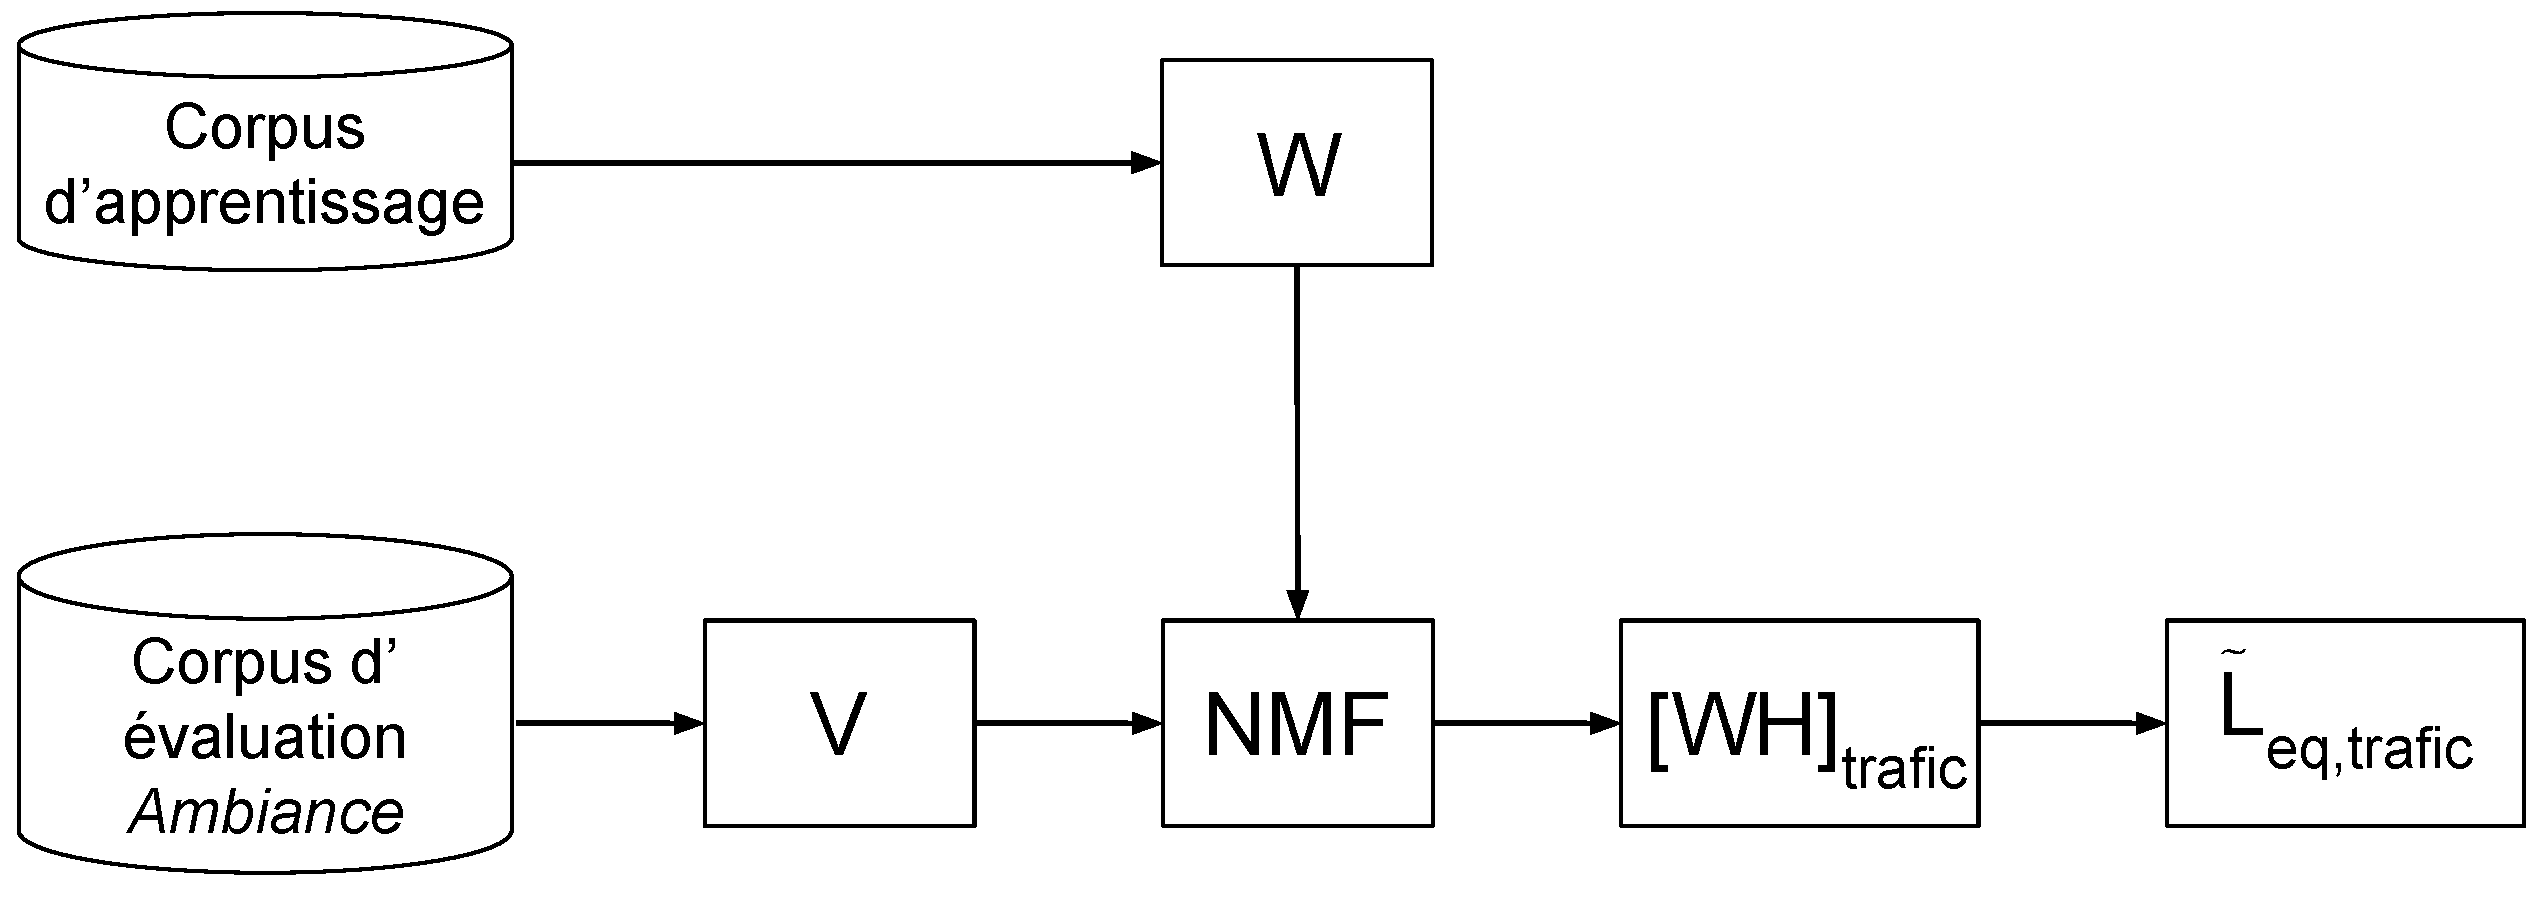
\includegraphics[width=0.7\linewidth]{./figures/NMF/NMF_ambiance.pdf}
\caption{Diagramme en blocs de l'estimateur NMF sur le corpus d'évaluation \textit{Ambiance}}
\label{fig:nmf_ambiance}
\end{figure}


\subsection{Apprentissage du dictionnaire}

Dans un premier temps, le dictionnaire $\mathbf{W}$ est construit, à partir du corpus d'apprentissage, composé d'enregistrements audio des passages des voitures Renault Scénic et Dacia Sandero sur la piste d'essais de l'Ifsttar. Ces 53 échantillons audio issus des enregistrements ne sont pas ceux utilisés dans la création des scènes sonores afin d'éviter tout problème de sur-apprentissage.

\begin{figure}[hbtp]
\centering
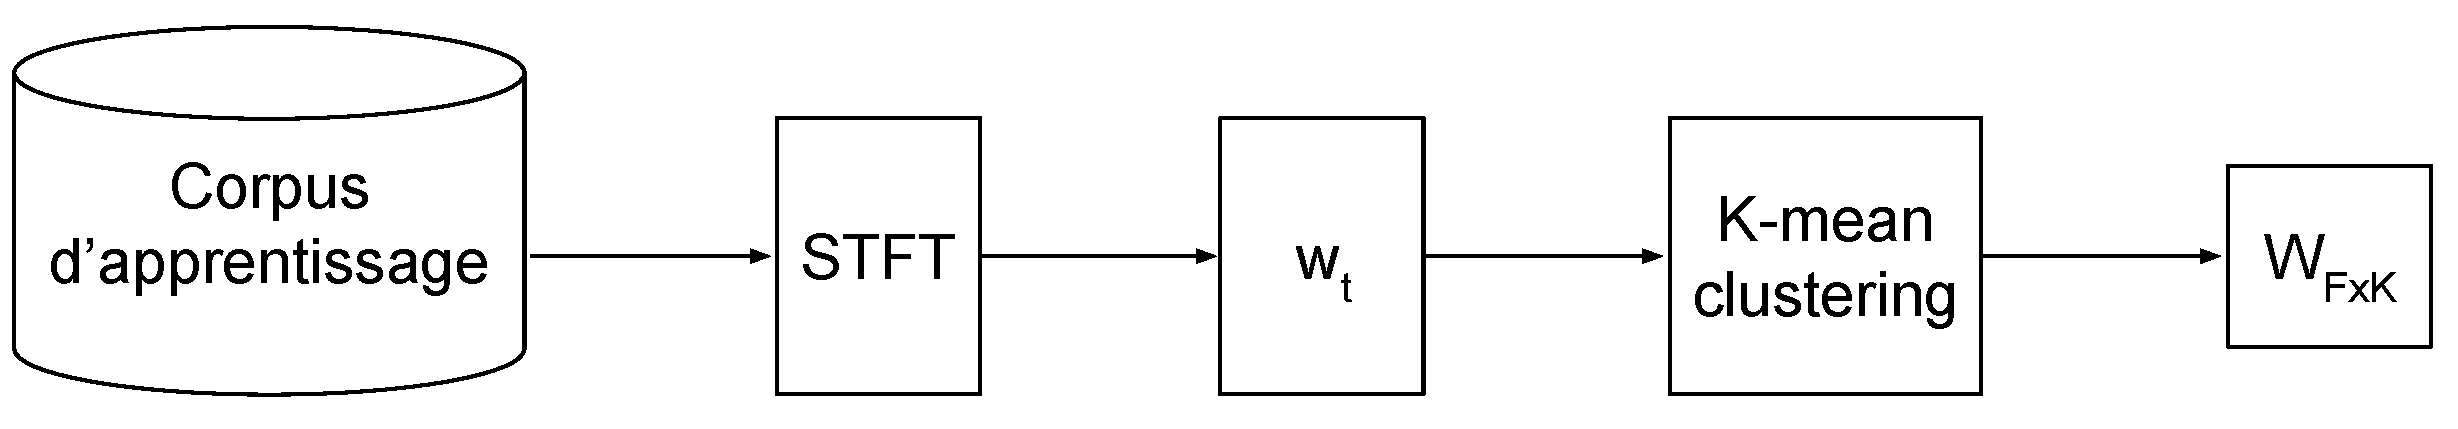
\includegraphics[width=.9\linewidth]{./figures/NMF/creation_dictionaire.pdf}
\caption{Diagramme en blocs de la création du dictionnaire}
\label{fig:creation_W}
\end{figure}


La constitution du dictionnaire est réalisée en trois étapes, résumée dans le diagramme en bloc en Figure \ref{fig:creation_W} : 
\begin{itemize}
\item chaque fichier audio est représenté au travers d'un spectrogramme, obtenu par une STFT (nombre de point $w = 2^{12}$ avec 50 $\%$ de recouvrement). Cette première étape permet d'obtenir pour chaque échantillon audio, de durée différente, le même nombre de point en fréquences.
\item Chaque spectrogramme est ensuite découpé en plusieurs trames temporelle de largeur $w_t \in \lbrace 0,5,~ 1,~ 2~\rbrace$ seconde(s). Dans chaque trame la valeur efficace (ou valeur \textit{rms} en anglais) sur chaque trame fréquentiel est calculé. Cet étape a pour but d'obtenir différents représentation des spectrogrammes initiaux avec une description du contenu spectrale plus ou moins fine. Dans le cas où $w_t = 0,5$ s, on obtient une description des spectres avec plus de détails que dans le cas où $w_t = 2$ s. Les étapes de ce processus sont résumés en Figure \ref{fig:decoupe_W} sur un extrait de 3 secondes.
\item Enfin, l'opération précédente générant un grand nombre de d'éléments (2218 pour $w_t$ = 0,5 s, 505 pour $w_t$ = 2 s), un algorithme de clustering $K$-mean est appliqué en vue de réduire ce nombre, d'éviter la présence d'informations redondantes et de fixer le nombre d'éléments à $K = \lbrace 25,~50,~100,~200 \rbrace$. Les $K$ centroïdes déterminés sont alors les éléments qui composent le dictionnaire $\mathbf{W}$.
\end{itemize}

En plus de ces étapes, on ajoute un cas où la valeur \textit{rms} est calculée sur l'ensemble des spectrogrammes ($w_t = all$). En cela, des 53 fichiers audio, 53 spectres sont générés. Cette opération permet de baser la construction du dictionnaire sur les enveloppes spectrales des fichiers audio \textit{trafic} et moins sur une description fine des spectres. Ces 53 spectres sont également soumis à l'algorithme de clustering mais avec cette fois, $K_{w_t = all} \in \lbrace 25,~ 50 \rbrace$. 

En tout, c'est 14 versions différentes du dictionnaire qui sont réalisées ($4\times 3 + 1 \times 2$ = 14).

\begin{figure}[hbtp]
\centering
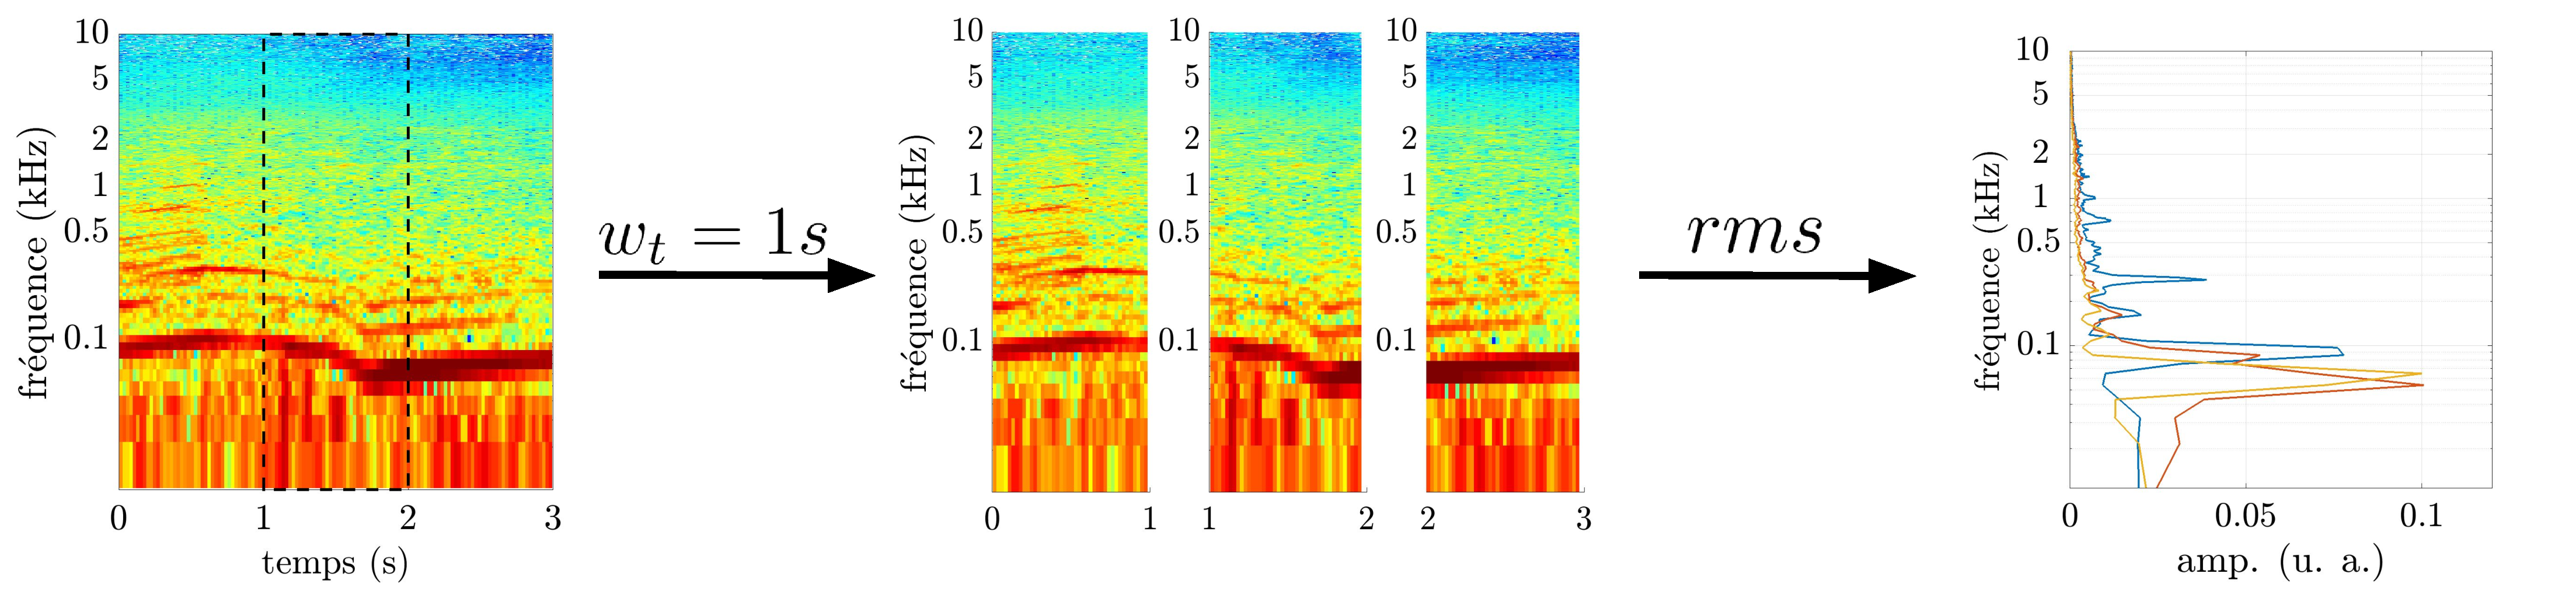
\includegraphics[width=\linewidth]{./figures/NMF/dictionaire_frame_FR.pdf} 
\caption{Création des éléments de $\mathbf{W}$ sur un extrait de 3 secondes du passage d'une voiture pour une largeur de la trame temporelle $w_t$ de 1 seconde. À gauche le spectrogramme du signal audio avec, en pointillés, une fenêtre de découpe de largeur $w_t$. Au centre, le signal est découpé en trois trames et dont les valeurs \textit{rms} sont ensuite calculés générant 3 spectres. }
\label{fig:decoupe_W}
\end{figure}

\subsection{Réalisation de la NMF}

Chaque dictionnaire $\mathbf{W}$ appris est soumis à l'estimateur NMF. Cette estimateur est lui-même basé sur plusieurs versions de la NMF décrit précédemment (voir chapitre \ref{chap:NMF})  : la NMF supervisée (NMF SUP), semi-supervisée (NMF SEM) et initialisée-seuillée (NMF IS). Pour chaque NMF, 3 $\beta$-divergences sont utilisées : la distance Euclidienne ($\beta = 2$) (voir partie \ref{part:dist_EUC}, la divergence de Kullback-Leibler ($\beta = 1$) (partie \ref{part:div_KL}), et la divergence d'Itakura-Saïto ($\beta = 0$) (partie \ref{part:div_IS}). 100 itérations sont en tout réalisées. 
La NMF SUP dépend seulement des différentes versions du dictionnaire appris et de $\beta$. Le signal trafic est estimé selon l'équation \ref{eq:WH_trafic} à partir de la matrice $\mathbf{H}$ obtenue.
Dans le cas de la NMF SEM, le dictionnaire appris compose la partie fixe $\mathbf{W_s}$. Le nombre d'éléments du dictionnaire libre $\mathbf{W_r}$ est alors fixé à 2 ($J = 2$). Le signal \textit{trafic} est ensuite déterminé par le relation \ref{eq:WSHs_trafic}. 
Enfin pour la NMF IS, les dictionnaires $\mathbf{W}$ correspondent aux dictionnaires initiaux $\mathbf{W_0}$ qui seront ensuite mis à jours. Le dictionnaire obtenu est ensuite soumis à l'étape d'extraction par seuillage qui implique également plusieurs facteurs expérimentaux : 

\begin{itemize}
\item la représentation de la distance $D_{\theta}(\mathbf{W_0}\Vert \mathbf{W})$ (linéaire ou bien exprimé au travers d'une fonction sigmoïde ($\lambda = 2$),
\item le type de seuillage appliqué (dur ou \textit{firm}),
\item les valeurs des différents seuils respectifs ($t_h$ pour le seuillage dur et $t_{f,1/2}$, les deux valeurs seuils pour le seuillage \textit{firm}). Des études préliminaires ont permis de réduire la plage des valeurs de ces seuils à $t_h \in \left[ 0,30~0,70 \right]$, $t_{f,1} \in \left[ 0,20~0,55 \right]$ et $t_{f,2} \in \left[ 0,35,~0,70 \right]$, chacun étant défini avec un pas de 0,01. Rappelons que pour le seuillage \textit{firm}, $t_{f,1} \leq t_{f,2}$.
\end{itemize}

Enfin, malgré la réduction du nombre d'éléments par l'algorithme $K$-mean, la taille des matrices $\mathbf{W}$ et $\mathbf{V}$ restent importantes en raison du nombre de trames fréquentielles ($F$ = 2048). En conséquence, ces deux matrices sont exprimées en bandes de tiers-d'octaves ce qui réduit les dimensions des matrices ($F_{1/3} = 29$). La manipulation des matrices est alors plus rapide qu'avec des bandes fines et permet donc un gain en temps de calculs. Cette représentation a également d'autres intérêts : 

\begin{itemize}
\item par son échelle logarithmique, elle permet de mieux décomposer les basses fréquences que les hautes fréquences ce qui permet de mieux focaliser la reconstruction du signal vers les bandes de fréquences d'intérêts.
\item Cette représentation est également couramment utilisée dans le domaine de l'acoustique urbaine et environnementale, à la différence des MFCC. En vue des applications prévue de ces outils (amélioration de la cartographie, estimation des sources sonores urbaines), c'est une représentation plus adaptée.
\end{itemize}

\begin{figure}[h]
\centering
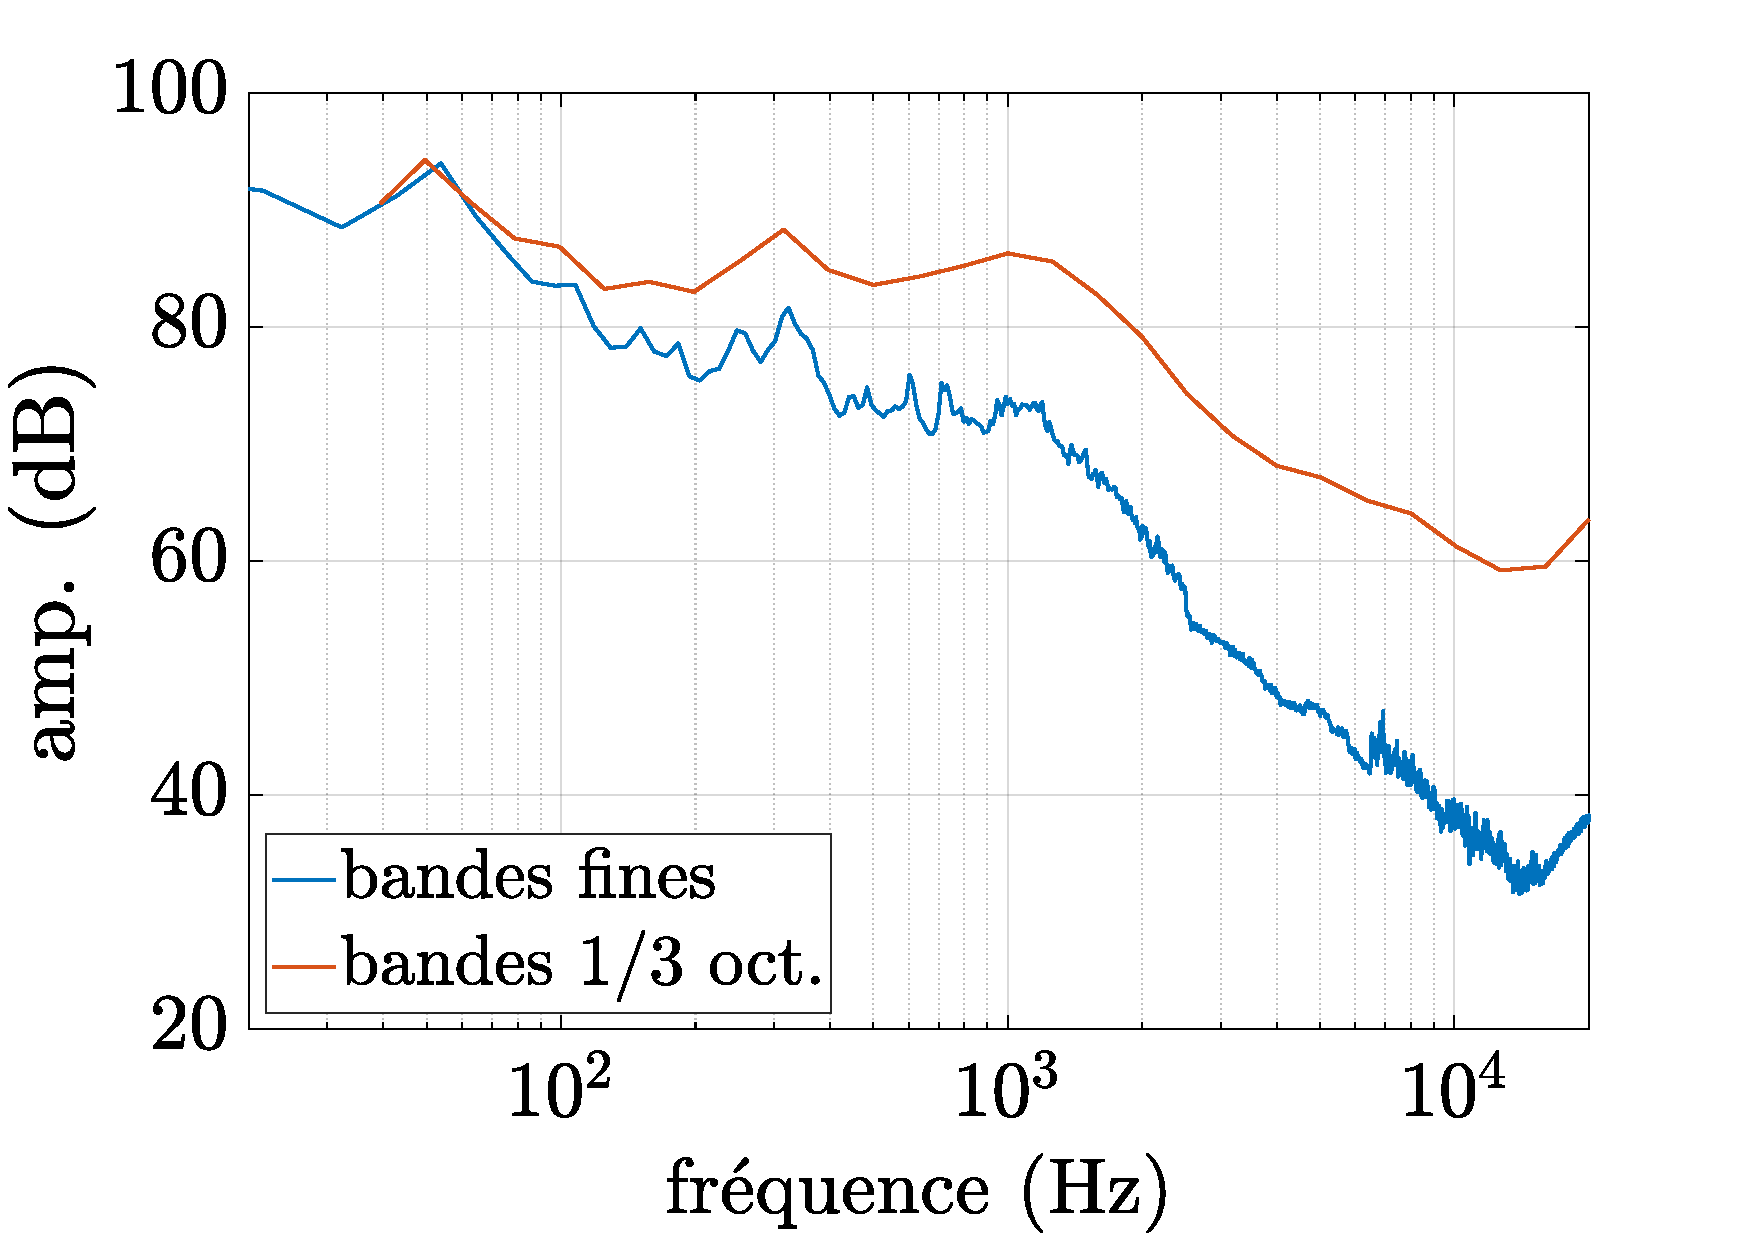
\includegraphics[width=0.5\linewidth]{./figures/NMF/bande_fine_tiers.pdf}
\caption{Spectre en fréquence du passage d'une voiture en bandes fines (2048 points) et en bandes de tiers d'octave (29 bandes)}
\end{figure}


\subsection{Résumé des facteurs expérimentaux}

De nombreux facteurs expérimentaux sont donc présents dans cette expérience, chacun ayant différentes modalités. Le Tableau \ref{tab:experimental_factorsNMF_ambiance} résume l'ensemble de ces paramètres qui implique les différents sous-corpus, valeurs du $TIR$ et facteurs expérimentaux lié aux estimateurs.


\begin{longenum}
	\item estimateur
	\begin{longenum}
		\item filtre
		\begin{longenum}
			\item $f_c$
		\end{longenum}
		\item NMF
		\begin{longenum}
			\item $\beta$
			\item $w_t$
			\item $K$
			\item méthode
			\begin{longenum}
				\item supervisée
				\item semi-supervisée
				\item initialisée-seuillée
				\begin{longenum}
					\item représentation
					\item seuillage
					\begin{longenum}
						\item dur avec $t_h$
						\item firme avec $t_{f,1} = $ et $t_{f,2}$
					\end{longenum}
				\end{longenum}
			\end{longenum}
		\end{longenum}
	\end{longenum}
\end{longenum}


\begin{table*}[h]
\centering
\caption{Facteurs expérimentaux et leur modalité utilisés pour le corpus \textit{Ambiance}.}
\begin{tabularx}{17.5cm}{L{3cm}@{}C{12cm}@{}C{2cm}@{}}
	\hline
    \textbf{\begin{tabular}[c]{@{}l@{}}facteur \\ expérimentaux \end{tabular}} & \textbf{modalités} & \begin{tabular}[c]{@{}C{2cm}@{}}\textbf{nombre de}\\ \textbf{modalités}\end{tabular}\\ \toprule
\end{tabularx}

\begin{tabularx}{17.5cm}{L{2.8cm}@{}@{}C{2cm}@{}@{}C{2cm}@{}@{}C{2cm}@{}@{}C{2cm}@{}@{}C{2cm}@{}@{}C{2.2cm}@{}C{2cm}}
   \textbf{sous-corpus} & alerte & animaux & climat &  humain & transport & mécanique & 6\\
\end{tabularx}

\begin{tabularx}{17.5cm}{L{2.8cm}@{}@{}C{2.435cm}@{}@{}C{2.435cm}@{}@{}C{2.435cm}@{}@{}C{2.435cm}@{}@{}C{2.435cm}@{}C{2cm}}
\rowcolor[HTML]{C0C0C0}
   $TIR$ (dB) & -12 & -6 & 0 & 6 & 12 & 5\\
\end{tabularx}

\begin{tabularx}{17.5cm}{L{3cm}@{}C{3cm}@{}@{}C{3cm}@{}@{}C{3cm}@{}@{}C{3cm}@{}C{2cm}@{}}
  \textbf{estimateur} & filtre passe bas & NMF SUP & NMF SEM & NMF IS & 4\\
\end{tabularx}

\begin{tabularx}{17.5cm}{L{3cm}@{}@{}C{1.7cm}@{}@{}C{1.7cm}@{}@{}C{1.7cm}@{}@{}C{1.7cm}@{}@{}C{1.7cm}@{}@{}C{1.7cm}@{}@{}C{1.78cm}@{}C{2cm}@{}}
\rowcolor[HTML]{C0C0C0}
   $\mathbf{f_c}$ (kHz) & 0,1 & 0,5 & 1 & 2 &  5 & 10 & 20 & 7\\
\end{tabularx}

\begin{tabularx}{17.5cm}{L{3cm}@{}C{3cm}@{}@{}C{3cm}@{}@{}C{3cm}@{}@{}C{3cm}@{}C{2cm}@{}}
    $\mathbf{w_t}$ (s)& 0,5 & 1 & 2 & \textit{all} & 4\\
\end{tabularx}

\begin{tabularx}{17.5cm}{L{3cm}@{}C{3cm}@{}@{}C{3cm}@{}@{}C{3cm}@{}@{}C{3cm}@{}C{2cm}@{}}
	\rowcolor[HTML]{C0C0C0}
    $\mathbf{K}$ & 25 & 50 & 100 & 200 & 4\\
\end{tabularx}

\begin{tabularx}{17.5cm}{L{3cm}@{}C{4cm}@{}@{}C{4cm}@{}@{}C{4cm}@{}C{2cm}@{}}
   $\mathbf{\beta}$ & 0 & 1 & 2 & 3\\
\end{tabularx}

\begin{tabularx}{17.5cm}{L{3cm}@{}C{6cm}@{}@{}C{6cm}@{}C{2cm}@{}}
	\rowcolor[HTML]{C0C0C0}
   \textbf{représentation} & linéaire & sigmoïde & 2\\
\end{tabularx}

\begin{tabularx}{17.5cm}{L{3cm}@{}C{12cm}@{}C{2cm}@{}}
	\textbf{seuil dur} $\mathbf{t_h}$ & de 0,30 à 0,60 avec un pas de 0.01 & 31\\
\end{tabularx}

\begin{tabularx}{17.5cm}{L{3cm}@{}C{12cm}@{}C{2cm}@{}}
	\rowcolor[HTML]{C0C0C0}
   \textbf{seuil firm} $\mathbf{t_{f,1}}$ & de 0,20 à 0,55 avec un pas de 0,01 & 36\\
\end{tabularx}

\begin{tabularx}{17.5cm}{L{3cm}@{}C{12cm}@{}C{2cm}@{}}
   \textbf{seuil firm} $\mathbf{t_{f,2}}$ & de 0,35 à 0,70 avec un pas de 0,01 & 36\\
   \bottomrule
\end{tabularx}
\label{tab:experimental_factorsNMF_ambiance}
\end{table*}

Pour l'estimateur filtre, c'est 210 combinaisons qui sont réalisées (6 sous-corpus $\times$ 5 $TIR$ $\times$ 7 $f_c$). Dans le cas de la NMF SUP et SEM, ce sont respectivement 1260 combinaisons qui sont calculées (6 sous-corpus $\times$ 5 $TIR$ $\times$ (3 $w_t$ $\times$ 4 $K$ + 1 $w_t$ $\times$ 2 $K$ ) $\times$ 3). Dans le cas de la NMF IS, ce nombre est beaucoup plus élevé en raison des nombreuses valeurs seuils (6 sous-corpus $\times$ 5 $TIR$ $\times$ (3 $w_t$ $\times$ 4 $K$ + 1 $w_t$ $\times$ 2 $K$ ) $\times$ 3 $\times$ 2 $\times$ (31 + ?????).

Les calculs sont réalisés sous le logiciel Matlab, avec l'aide de l'outil expLanes\footnote{\url{http://mathieulagrange.github.io/expLanes/}} qui permet la réalisation d'expériences numérique, de gérer la distribution des nombreux facteurs expérimentaux et leur modalités et de collecter les nombreux résultats générés. L'ordinateur menant les calculs est équipé d'un processeur Inter Core i7 (CPU 2,40 GHz).

\section{Résultats}

\subsection{Performance de l'estimateur \textit{baseline}}

Les résultats issus de l'estimateur \textit{baseline} sont d'abord présentés. Dans un premier temps, les erreurs $MAE_g$ émises par les estimations réalisées par chaque filtre sur l'ensemble du corpus sont résumées dans le Tableau \ref{tab:resuls_ambiance_filtre} ainsi que les erreurs $MAE_{TIR}$.  

\begin{table}[h]
\centering
\caption{Erreur $MAE$ de l'estimateur \textit{baseline} selon $f_c$ sur l'ensemble du corpus \textit{Ambiance} et pour chaque TIR. En gras-rouge l'erreur $MAE_g$ la plus faible, en gras-noir, les erreurs $MAE_{TIR}$ les plus faibles selon les fréquences $f_c$.}
\label{tab:resuls_ambiance_filtre}
\resizebox{\textwidth}{!}{%
\begin{tabular}{lcccccc}
\toprule
$f_c$ (Hz) & $MAE_g$ & $MAE_{-12}$ & $MAE_{-6}$ & $MAE_{0}$ & $MAE_{6}$ & $MAE_{12}$ \\ 
\midrule
 100 & 3,21 ($\pm$ 1,06) & \textbf{4,55 ($\pm$ 1,55)} & \textbf{2,92 ($\pm$ 0,42)} & 2,36 ($\pm$ 0,71) & 2,97 ($\pm$ 0,41) & 3,25 ($\pm$ 0,32)\\
 500 & \textbf{\textcolor{red}{2,89 ($\pm$ 2,84)}} & 7,39 ($\pm$ 3,00) & 3,44 ($\pm$ 1,65) & \textbf{1,17 ($\pm$ 0,24)} & 1,03 ($\pm$ 0,26) & 1,45 ($\pm$ 0,13) \\  
 1000 & 3,36 ($\pm$ 3,63) & 9,44 ($\pm$ 2,03) & 4,78 ($\pm$ 1,34) & 1,62 ($\pm$ 0,54) & \textbf{0,36 ($\pm$ 0,10)} & 0,61 ($\pm$ 0,06) \\ 
 2000 & 3,83 ($\pm$ 4,01) & 10,30 ($\pm$ 1,57) & 5,65 ($\pm$ 1,05) & 2,25 ($\pm$ 0,49) & 0,62 ($\pm$ 0,15) & \textbf{0,11 ($\pm$ 0,02)}\\ 
 5000 & 4,51 ($\pm$ 4,43) & 11,95 ($\pm$ 0,20) & 6,70 ($\pm$ 0,16) & 2,82 ($\pm$ 0,10)  & 0,87 ($\pm$ 0,04) & 0,20 ($\pm$ 0,02)\\ 
10000 & 4,64 ($\pm$ 4,51) & 12,19 ($\pm$ 0,08) & 6,90 ($\pm$ 0,07) & 2,95 ($\pm$ 0,05) & 0,92 ($\pm$ 0,02) & 0,22 ($\pm$ 0,01)\\ 
20000 & 4,69 ($\pm$ 4,52) & 12,25 ($\pm$ 0,05) & 6,96 ($\pm$ 0,05) & 3,00 ($\pm$ 0,03) & 0,97 ($\pm$ 0,01) & 0,26 ($\pm$ 0,00)\\ 
\bottomrule
\end{tabular}}
\end{table}

La plus faible erreur $MAE_g$ sur l'intégralité du corpus est obtenue pour une fréquence de coupure $f_c$ de 500 Hz ($MAE_g$ = 2,89 ($\pm$ 2,84)).
\`A l'inverse, c'est naturellement pour la fréquence de coupure de 20 kHz que l'erreur est la plus importante puisque l'intégralité des sources sonores sont considérés ($MAE_g$ = 4,69 ($\pm$ 4,52). 
En détaillant les erreurs $MAE_{TIR}$, on constante que la fréquence de coupure correspondant à l'erreur minimale évolue en fonction de la prédominance du trafic : plus le $TIR$ augmente, plus la fréquence de coupure $f_c$ augmente.
Naturellement, avec l'augmentation de la présence des voitures, il est nécessaire d'augmenter la fréquence $f_c$ afin de conserver le plus possible l'énergie sonore de cette source. \`A l'opposé, lorsque le $TIR$ est plus faible, le filtre le plus performant sera celui qui est susceptible soit d'éliminer suffisamment d'énergie pour ne pas prendre en considération les sources sonores interférantes, soit de trouver un compromis entre l'énergie conservée de la classe de son interférante et du trafic.

Dans le cas du filtre $f_c$ = 500 Hz,  on détaille les erreurs par sous-corpus et TIR (Figure \ref{fig:filtre_amb_tir}). 

\begin{figure}[h]
\centering
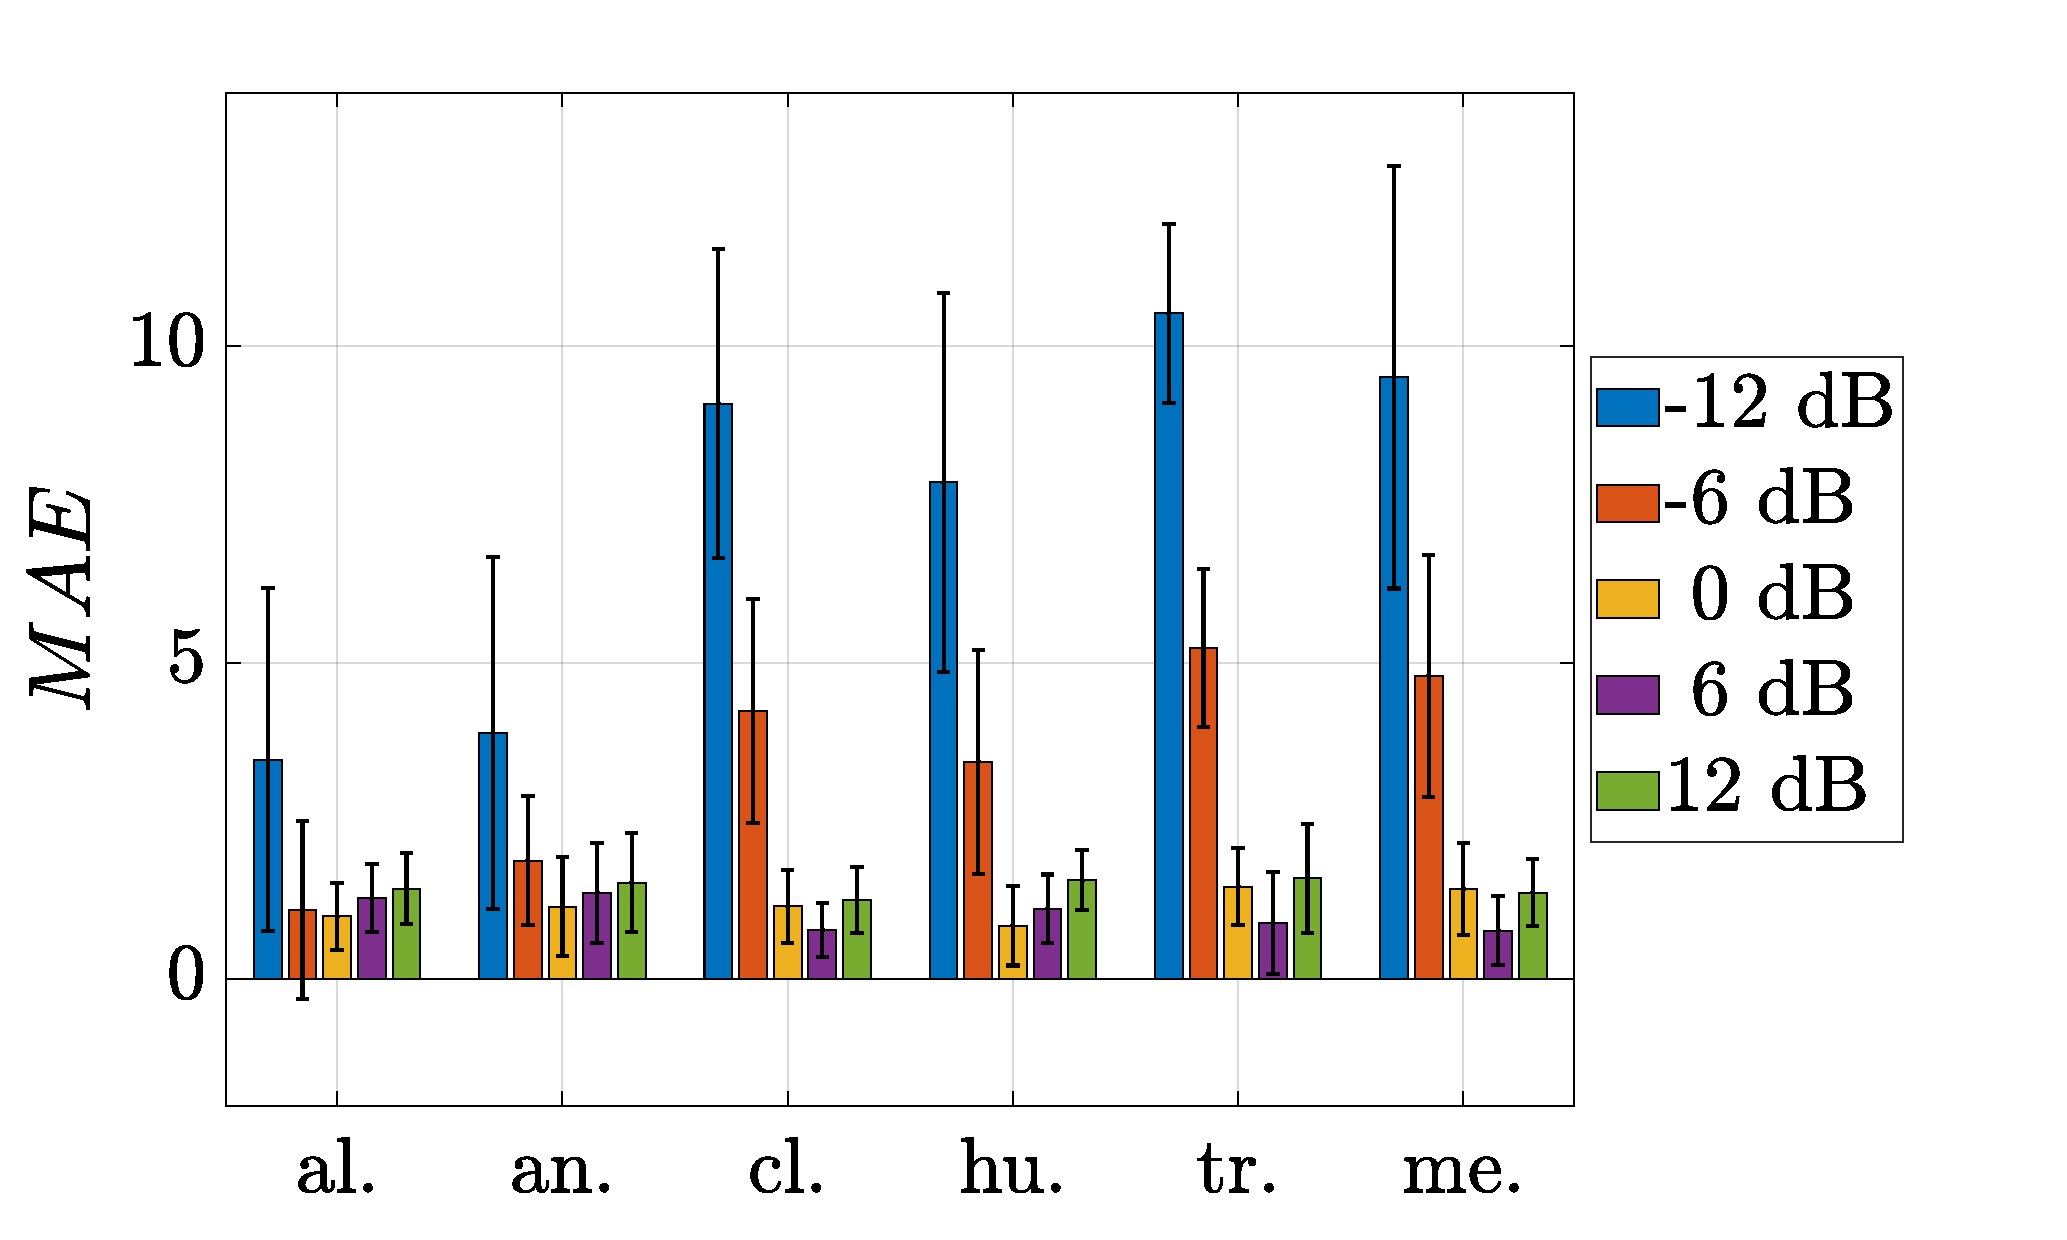
\includegraphics[width=0.7\linewidth]{./figures/resultats/amb_filtre_500_bar.pdf}
\caption{Erreur $MAE$ pour chaque sous-corpus et chaque TIR pour l'estimateur filtre passe-bas à la fréquence de coupure $f_c$ = 500 Hz.}
\label{fig:filtre_amb_tir}
\end{figure}

On observe de fortes erreurs pour les faibles TIR (-12 dB et -6 dB) notamment pour les sous-corpus \textit{climat}, \textit{humain}, \textit{transport} et \textit{mécanique}. Ces sous-corpus contiennent des composantes situées dans les basses fréquences plus importantes. L'erreur du filtre à 500 Hz est alors du à la présence d'une partie de l'énergie de la classe interférante. Dans ces $TIR$, le filtre se révèle plus efficace pour les sous-corpus \textit{alerte} et \textit{animaux}, puisque les spectres sonores sont plus aigus et donc mieux filtrés.
Avec l'augmentation du $TIR$, lorsque le trafic devient prédominant, l'erreur devient faible ($MAE < 2 dB$) avec toutefois, une augmentation de l'erreur $TIR$ =  6 dB et $TIR$ = 12 dB pour chaque sous-corpus. Cette erreur est ici due à la suppression de trop importante de la composante \textit{trafic}. Dans le cas extrême de $f_c$ = 20 kHz (Figure \ref{fig:filtre_amb_tir_20k}), cette erreur disparait logiquement : la source trafic étant principale, en conservant toute l'énergie sonore, l'estimation du trafic en devient correcte. Mais dans les cas où le TIR est négatif, l'erreur augmente significativement. Cette erreur revient finalement à la somme des niveaux sonores des classes.

\begin{figure}[h]
\centering
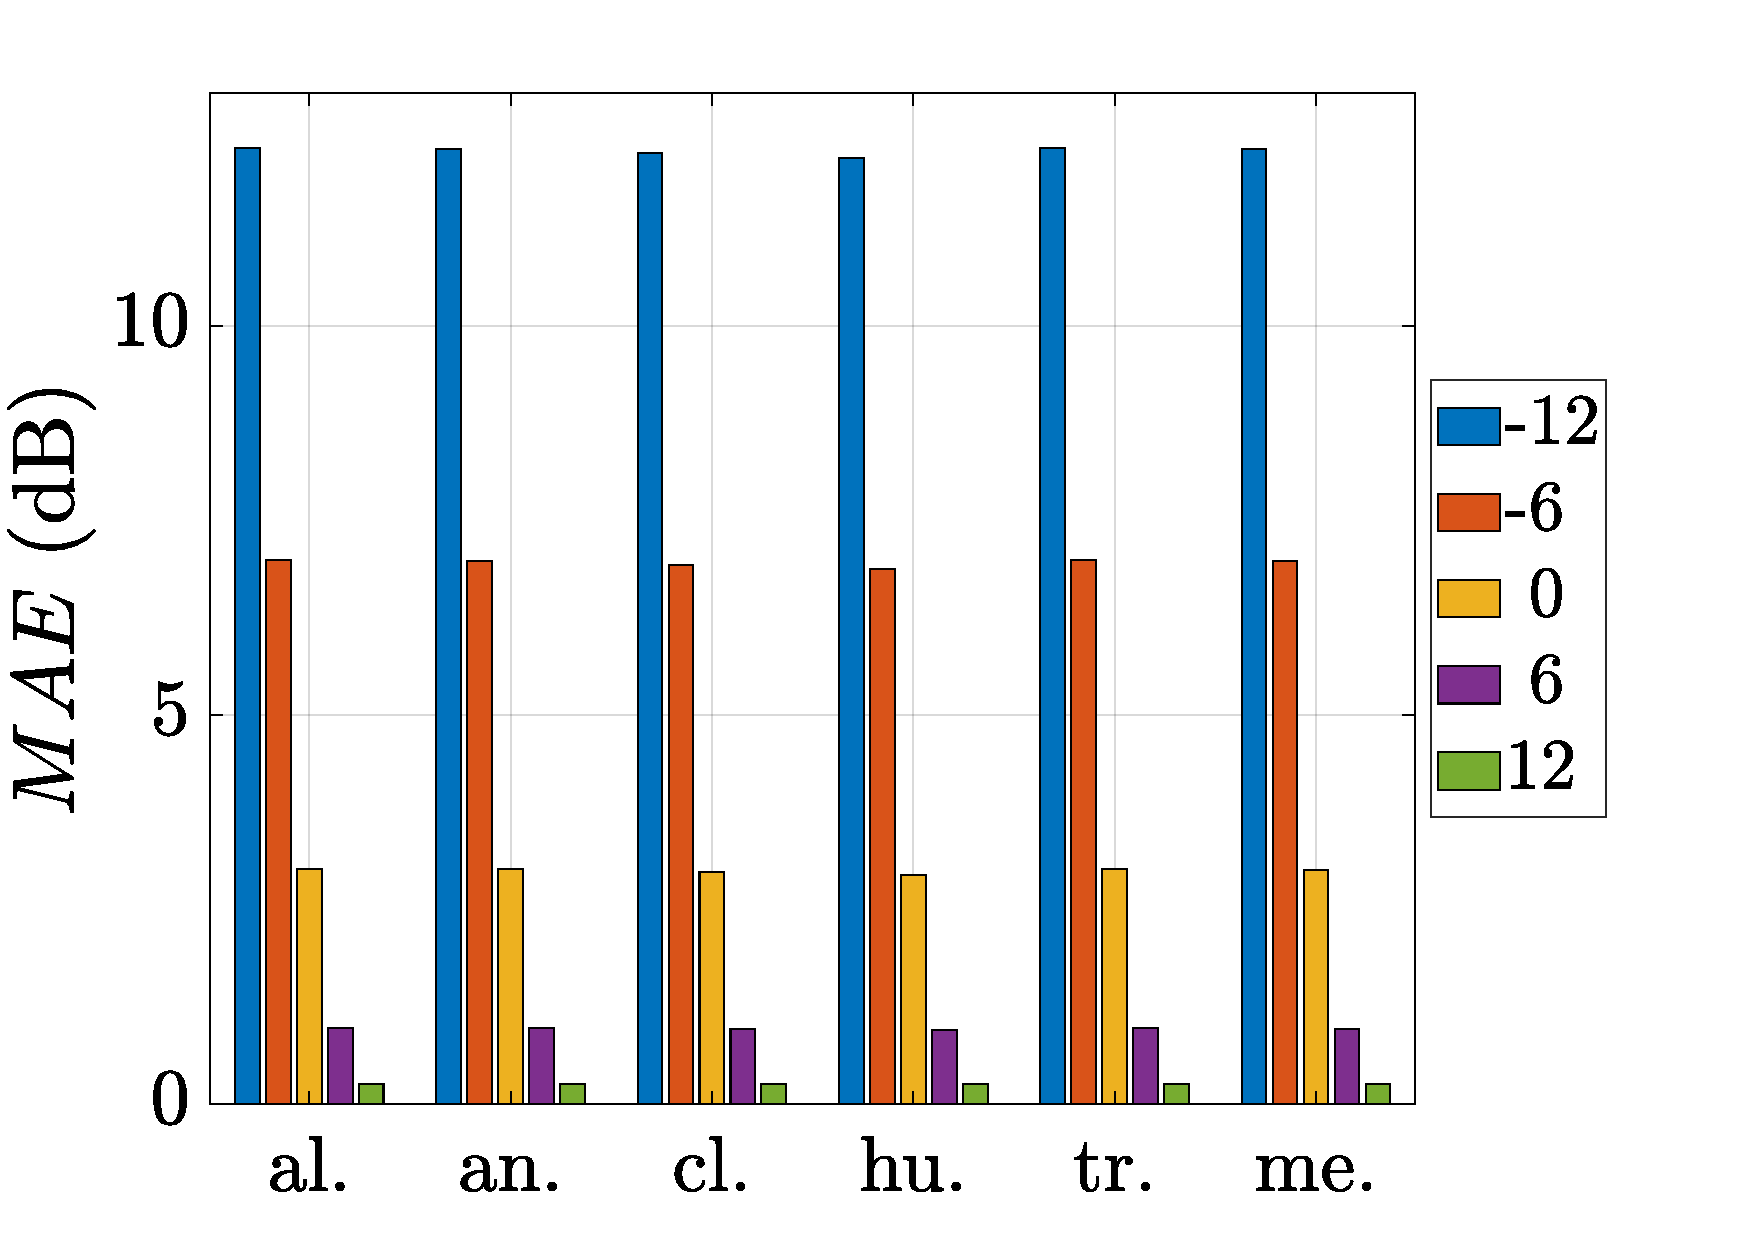
\includegraphics[width=0.7\linewidth]{./figures/resultats/amb_filtre_20k_bar.pdf}
\caption{Erreur $MAE$ pour chaque sous-corpus et chaque TIR pour l'estimateur filtre passe-bas à la fréquence de coupure $f_c$ = 20 kHz}
\label{fig:filtre_amb_tir_20k}
\end{figure}

\begin{subequations}
\begin{align}
\tilde{L}_{eq,trafic,tir,i} &= L_{eq,globale,tir,i}\\
 & = 10\times \log_{10}\left(10^{L_{eq,trafic,tir,i}/10}+10^{L_{eq,interferant,tir,i}/10}\right)
\end{align}
\end{subequations}


En résumé, le filtre passe-bas avec une fréquence de coupure $f_c$ de 500 Hz est donc le filtre qui est le plus efficace sur l'ensemble du corpus qui n'est toutefois pas le plus efficace sur chaque TIR. Celui-ci correspond plus à un compromis entre l'énergie rejetée dans les faibles $TIR$ et l'énergie conservée dans les haut $TIR$. 

\subsection{Résultats de la NMF}
On résume les erreurs produites par les différentes versions de la NMF d'abord selon l'erreur $AME_g$ pui, dans un second temps, les erreurs $MAE_{TIR}$ et $MAE$ sont observées pour chaque méthode de NMF proposant les plus faibles erreurs.

\subsubsection{Erreur $MAE_g$ de la NMF}

Le nombre de combinaison de modalité entre les différentes facteurs expérimentaux étant important, on résume, dans un premier temps, les erreurs $MAE_g$ les plus faibles produites par la NMF SUP et SEM selon chaque valeur de $\beta$ avec les modalités correspondantes. Puis, dans le cas de la NMF IS, l'influence de la représentation de la distance et du type de seuil est observé.

\begin{table}[h]
\caption{Erreur $MAE_g$ de la NMF SUP et NMF SEM pour le corpus d'évaluation \textit{Ambiance}}
\label{tab:erreur_ambiance_SUP_SEM}
\centering
\begin{tabular}{L{2.2cm}C{1.2cm}C{1.2cm}C{1.2cm}C{1.2cm}C{2.5cm}}
\toprule
 & $f_c$ & $\beta$ & $w_t$ & $K$ & $MAE_g$ \\ \toprule
\multirow{2}{*}{filtre PB} & 20 & - & - & - & 4,69 ($\pm$ 4,52) \\
 & 0,5 & - & - & - & 2,89 ($\pm$ 2,84) \\
 \midrule
\multirow{3}{*}{NMF SUP} & - & 0 & \textit{all} & 50 & 4,43 ($\pm$ 4,30) \\
 & - & 1 & \textit{all} & 50 & 3,51 ($\pm$ 3,74) \\
 & - & 2 & 0,5 & 25 & 2,92 ($\pm$ 3,23)  \\
 \midrule
\multirow{3}{*}{\textbf{NMF SEM}} & - & 0 & 1 & 200 & 2,51 ($\pm$ 1,13) \\
 & - & \textbf{1} & \textbf{1} & \textbf{200} & \textbf{\textcolor{red}{2,40 ($\pm$ 1,16)}} \\
 & - & 2 & 1 & 200 & 2,47 ($\pm$ 1,27)\\ \bottomrule
\end{tabular}
\end{table}

La NMF SUP offre des estimations moins bonnes que l'estimateur \textit{baseline} pour $f_c$ = 500 Hz pour chaque valeur de $\beta$. L'erreur la plus faible y est atteinte pour $\beta$ = 2 avec une erreur similaire au filtre. 
Dans le cas de la divergence IS et KL, le dictionnaire comprend un faible nombre d'élément avec $w_t = all$, qui correspond au cas où le dictionnaire contient des enveloppes spectrales. Ces modalités traduit la nécessité pour cette méthode d'avoir un dictionnaire qui généralise au mieux les différentes cas rencontrés puisque le dictionnaire est fixe. Le dictionnaire de la NMF SUP avec $\beta$ = 2 est le plus petit ($\mathbf{K}$ = 25 éléments) mais basé sur une description fine du dictionnaire ($w_t = 0,5$ s).
La NMF SEM offre des erreurs plus faibles que l'estimateur \textit{baseline} pour les 3 valeurs de $\beta$ avec des écarts-types réduits. Dans les 3 cas, le dictionnaire est basé sur les mêmes paramètres avec ici un grand nombre d'éléments ($K$ = 200). 
La différence entre la NMF SEM et SUP réside dans la présence du dictionnaire libre $W_r$ dans la NMF SEM qui permet plus d'adaptabilité. La NMF étant constitué que d'un dictionnaire fixe composé d'éléments \textit{trafic}, elle est susceptible d'être plus contraint dans son fonctionnement.\\

La NMF IS étant une nouvelle forme de NFM proposée ici, plusieurs pistes sont explorées afin de trouver une configuration optimale. Dans un premier temps, la représentation de la distance $D_{\theta}(\mathbf{W_0}\Vert \mathbf{W})$ naturelle ou exprimée au travers d'une fonction sigmoïde est observée dans le Tableau \ref{tab:erreur_ambiance_IS} selon un seuillage dur. 

\begin{table}[h]
\centering
\caption{Erreurs $MAE_g$ de la NMF IS pour le corpus d'évaluation \textit{Ambiance} selon la représentation linéaire ou sigmoïde de la distance $D_{\theta}(\mathbf{W_0}\Vert \mathbf{W})$.}
\label{tab:erreur_ambiance_IS}
\begin{tabular}{C{1.2cm}C{1.2cm}C{1.2cm}C{2.5cm}C{1.2cm}C{2.5cm}}
\toprule
\multicolumn{1}{l}{$\beta$} & $w_t$ & $K$ & représentation & $t_h$ & $MAE_g$ \\ \toprule
\multirow{2}{*}{0} & 500 & 200 & linéaire & 0,47 & 2,26 ($\pm$ 2,15) \\
 & 500 & 200 & sigmoïde & 0,62 & 2,27 ($\pm$ 1,94) \\ \midrule
\multirow{2}{*}{\textbf{1}} & \textbf{500} & \textbf{200} & \textbf{linéaire} & \textbf{0,41} & \textbf{\textcolor{red}{2,16 ($\pm$ 2,11)}} \\
 & 500 & 200 & sigmoïde & 0,60 & 2,14 ($\pm$ 2,19) \\ \midrule
\multirow{2}{*}{2} & 500 & 200 & linéaire & 0,36 & 2,29 ($\pm$ 2,40)\\
 & 500 & 200 & sigmoïde &  0,59 & 2,29 ($\pm$ 2,45)  \\
\bottomrule
\end{tabular}
\end{table}

Dans un premier temps, on remarque que, comme la NMF SEM, que la méthode privilégie un nombre d'éléments dans le dictionnaire important ($K$ = 200). De plus, le choix de la représentation de $D_{\theta}(\mathbf{W_0}\Vert \mathbf{W})$ n'influe pas sur la formation du dictionnaire puisque $w_t$ et $K$ restent constants.
L'erreur $MAE_g$ selon la représentation de $D_{\theta}$ est très influencé : les erreurs restent les mêmes, seul les seuils doivent être adaptés. La fonction sigmoïde déformant $D_{\theta}$ , les valeurs du seuil doivent être ré-hausser.
De ces premiers résultats, une représentation linéaire de $D_{\theta}$ est choisie pour la suite. 

De cette représentation linéaire de $D_{\theta}$, le type de seuillage est observé. Les erreurs $MAE_g$ sont présentées dans le Tableau \ref{tab:erreur_ambiance_IS_seuil} pour chaque valeur de $\beta$. Là encore, le dictionnaire optimale reste le même et n'est pas influencé par le choix de la technique du seuillage. On constate que les valeurs de seuils $t_{f,1}$ et $t_{f,2}$ encadre la valeur du seuil dur $t_h$. Si cet encadrement est important pour $\beta = 2$, pour $\beta \in \lbrace 0,~1 \rbrace$ cet encadrement est faible. Sur l'ensemble des cas, l'apport du seuillage \textit{firm} est quasi nul par rapport au seuillage dur.\\

\begin{table}[h]
\centering
\caption{Erreur $MAE$ de la NMF IS pour le corpus d'évaluation \textit{Ambiance} selon un seuillage dur ou \textit{firm}.}
\label{tab:erreur_ambiance_IS_seuil}
\begin{tabular}{C{1.2cm}C{1.2cm}C{1.2cm}C{1.2cm}C{1.2cm}C{1.2cm}C{2.5cm}}
\toprule
\multicolumn{1}{l}{$\beta$} & $w_t$ & $K$ & $t_h$ & $t_{f,1}$ & $t_{f_2}$ & $MAE$ \\ \toprule
\multirow{2}{*}{0} & 500 & 200 & 0,47 & - & - & 2,26 ($\pm$ 2,15) \\
 & 500 & 200 & - & 0,44 & 0,50 & 2,25 ($\pm$ 2,14)  \\ \midrule
\multirow{2}{*}{\textbf{1}} & 500 & 200 & 0,41 & - & - & 2,16 ($\pm$ 2,11) \\
 & \textbf{500} & \textbf{200} & - & \textbf{0,39} & \textbf{0,42} & \textbf{\textcolor{red}{2,15 ($\pm$ 2,17)}}  \\ \midrule
\multirow{2}{*}{2} & 500 & 200 &  0,36 & - & - & 2,29 ($\pm$ 2,40)\\
 & 500 & 200 & - & 0,24 & 0,48 & 2,25 ($\pm$ 2,45)  \\ 
 \bottomrule
\end{tabular}
\end{table}

En conséquence, puisque l'influence du seuillage \textit{firm} reste très faible et que la représentation de $D_{\theta}$ via une fonction sigmoïde ne diminue pas les erreurs, en vue de simplifier l'étude, on ne considère que le cas d'une NMF IS avec une représentation linéaire de $D_{\theta}$ et un seuillage dur. 

\subsubsection{Erreur $MAE_{TIR}$ et $MAE$}

De ces premiers résultats on retient donc une combinaison de modalités pour chaque NMF : 

\begin{itemize}
\item NMF SUP avec $\beta$ = 2, $K$ = 25, et $w_t$ = 0,5 s, 
\item NMF SEM avec $\beta$ = 1, $K$ = 200, et $w_t$ = 1 s, 
\item NMF IS avec $\beta$ = 1, $K$ = 200, $w_t$ = 0,5 s et $t_h$ = 0,41.\\
\end{itemize}

À partir de ces 3 estimateurs, leur erreurs selon chaque $TIR$, $MAE_{TIR}$ sont exprimés dans le Tableau \ref{tab:mae_tir_ambiance}. À ces résultats sont ajoutées ceux de l'estimateur baseline pour $f_c$ = 500 Hz et $f_c$ = 20 kHz. En gras-rouge, les erreurs $MAE_{TIR}$ les plus faibles, en gras-noir les erreurs générées par les NMF inférieures à la baseline $f_c = 500 Hz$.

\begin{table}[h]
\centering
\caption{Erreurs $MAE_{TIR}$ selon les combinaisons optimales de la NMF SUP, SEM et IS.}
\label{tab:mae_tir_ambiance}
\resizebox{\textwidth}{!}{%
\begin{tabular}{L{4cm}C{2.5cm}C{2.5cm}C{2.5cm}C{2.5cm}C{2.5cm}}
\toprule
méthode & -12 & -6 & 0 & 6 & 12 \\ \toprule
filtre PB, $f_c$ = 20 kHz & 12,25 ($\pm$ 0,05) & 6,96 ($\pm$ 0,05) & 3,00 ($\pm$ 0,03) & 0,97 ($\pm$ 0,01) & \textbf{\textcolor{red}{0,26 ($\pm$ 0,00)}}\\
filtre PB, $f_c$ = 0,5 kHz & 7,39 ($\pm$ 3,00) & 3,44 ($\pm$ 1,65) & \textbf{\textcolor{red}{1,17 ($\pm$ 0,24)}} & 1,03 ($\pm$ 0,26) & 1,45 ($\pm$ 0,13) \\ \midrule
NMF SUP & 8,34 ($\pm$ 2,05) & 4,00 ($\pm$ 1,37) & 1,20 ($\pm$ 0,59) & \textbf{\textcolor{red}{0,30 ($\pm$ 0,16)}} & \textbf{0,73 ($\pm$ 0,06) } \\
NMF SEM & \textbf{\textcolor{red}{3,34 ($\pm$ 1,95)}} & \textbf{\textcolor{red}{1,60 ($\pm$ 0,59)}} & 1,52 ($\pm$ 0,45) & 2,50 ($\pm$ 0,34) & 3,03 ($\pm$ 0,23)  \\
NMF IS & \textbf{5,22 ($\pm$ 2,62)} & \textbf{2,72 ($\pm$ 1,24)} & 1,26 ($\pm$ 0,35) & \textbf{0,75 ($\pm$ 0,34)} & \textbf{0,83 ($\pm$ 0,23)} \\ \bottomrule
\end{tabular}}
\end{table}

De la même manière que pour l'estimateur filtre dans le Tableau \ref{tab:resuls_ambiance_filtre}, la méthode la plus efficace sur l'ensemble du corpus n'est pas forcément la méthode la plus efficace pour chaque $TIR$. Ici, la NMF IS, si elle est pour 4 $TIR$ inférieure à la baseline, n'est pour autant jamais la méthode qui propose l'erreur la plus faible ! Pour $TIR \in \lbrace -12, -6 \rbrace$, la NMF SEM est la plus performante, alors que pour $TIR\in \lbrace 6, 12 \rbrace$, la NMF SUP supplante les deux autres méthodes. Dans le cas ou $TIR = 12 dB$ c'est finalement le filtre $f_c$ = 20 kHz, qui se trouve être la méthode la plus performante. Toutefois, la NMF IS est la seule à être systématiquement inférieure à la baseline (hormis à $TIR = 0$ dB) et même si elle n'est pas systématiquement la plus performante est celle qui s'adapte le mieux aux différentes valeurs du $TIR$.\\

\begin{figure}%
\centering
\subfigure[Erreurs $MAE$ pour la NMF SUP.]{%
\label{fig:TIR_class_sup}%
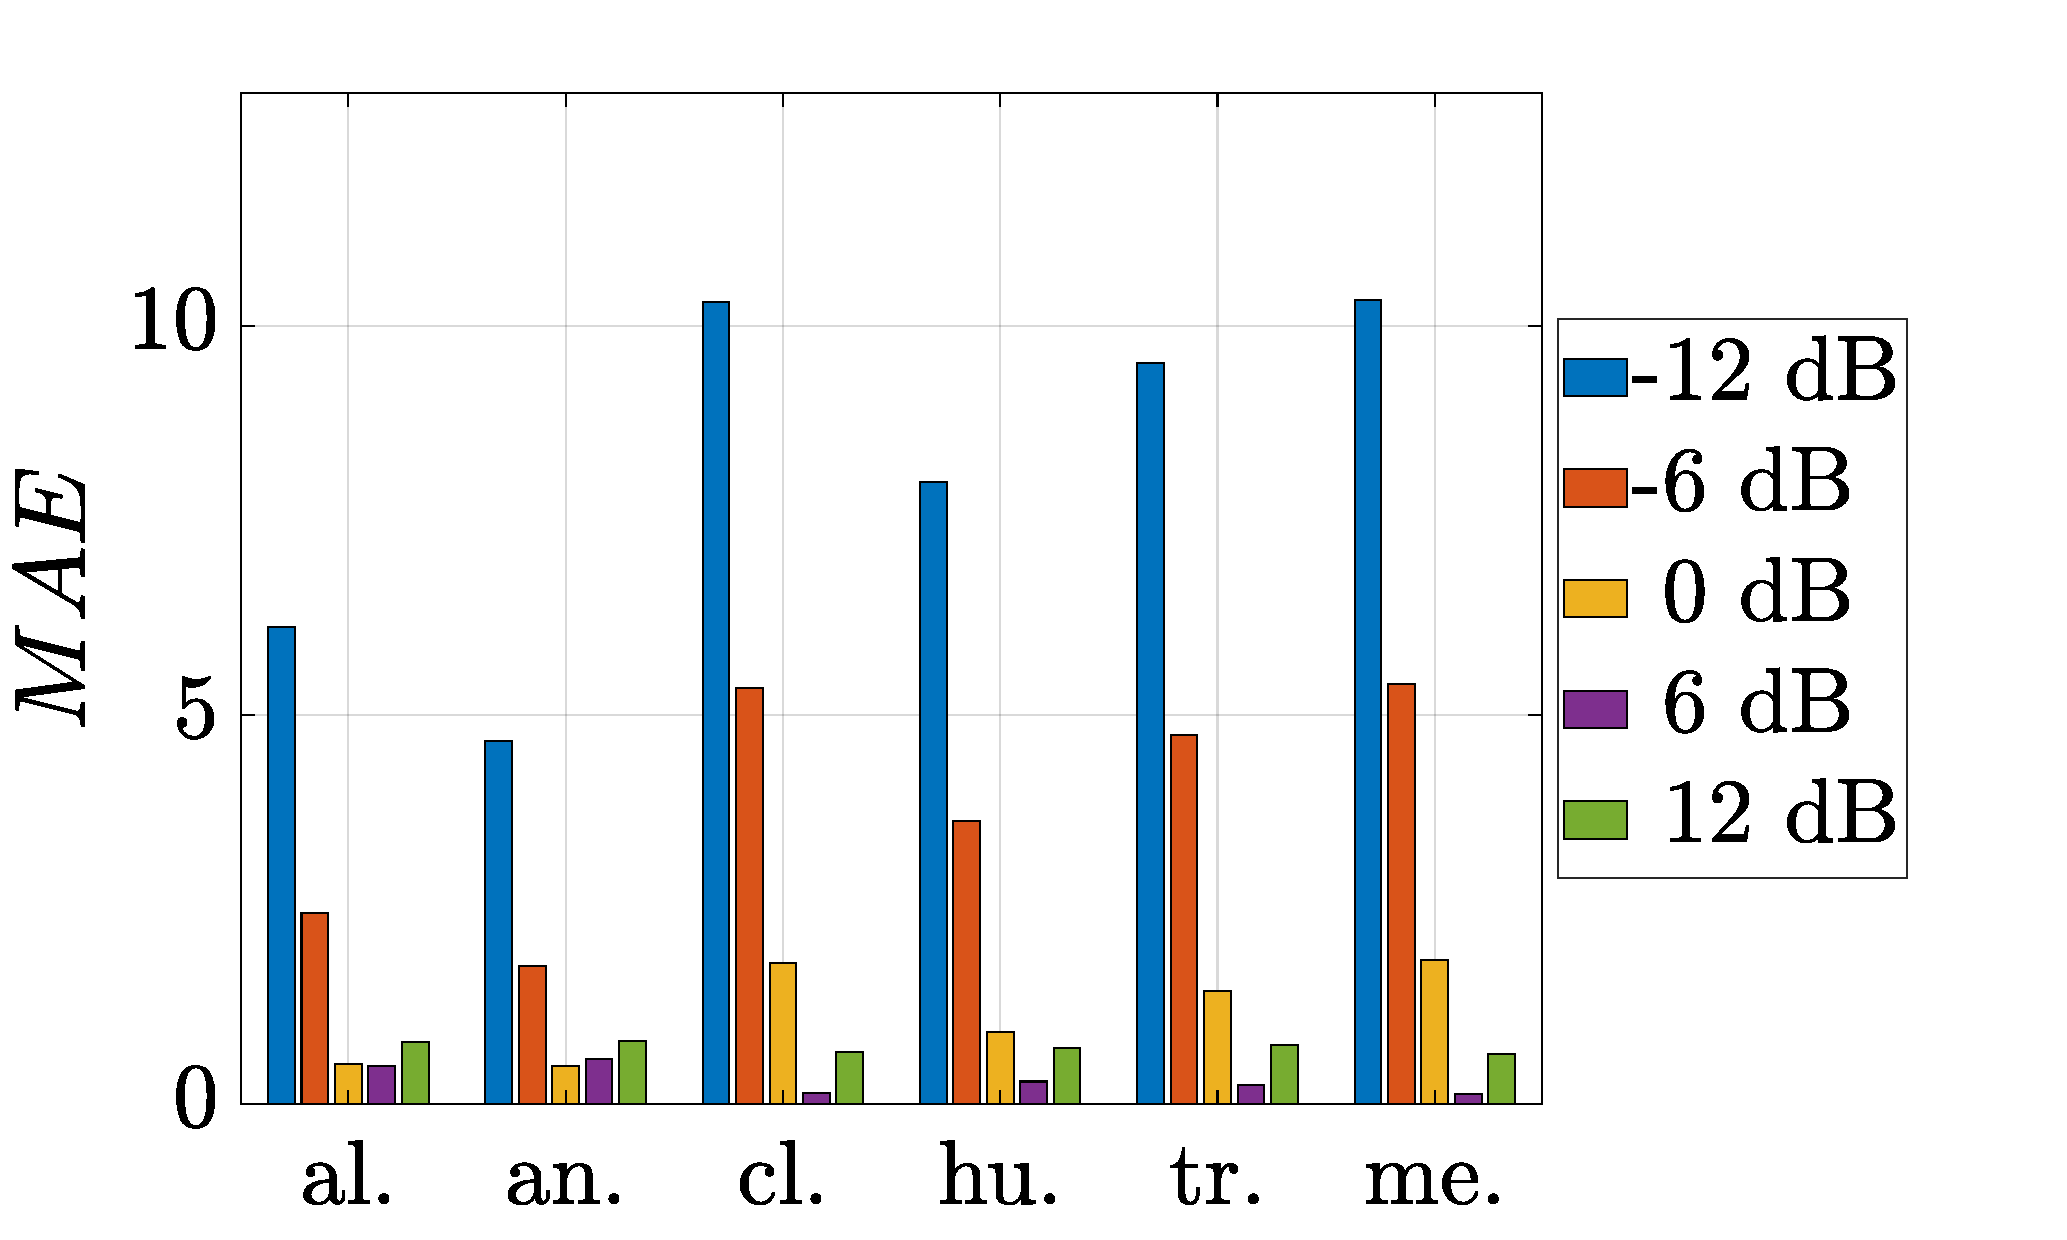
\includegraphics[width=0.60\linewidth]{./figures/resultats/ambiance_sup_bar.pdf}}%
\qquad
\subfigure[Erreurs $MAE$ pour la NMF SEM.]{%
\label{fig:TIR_class_semi}%
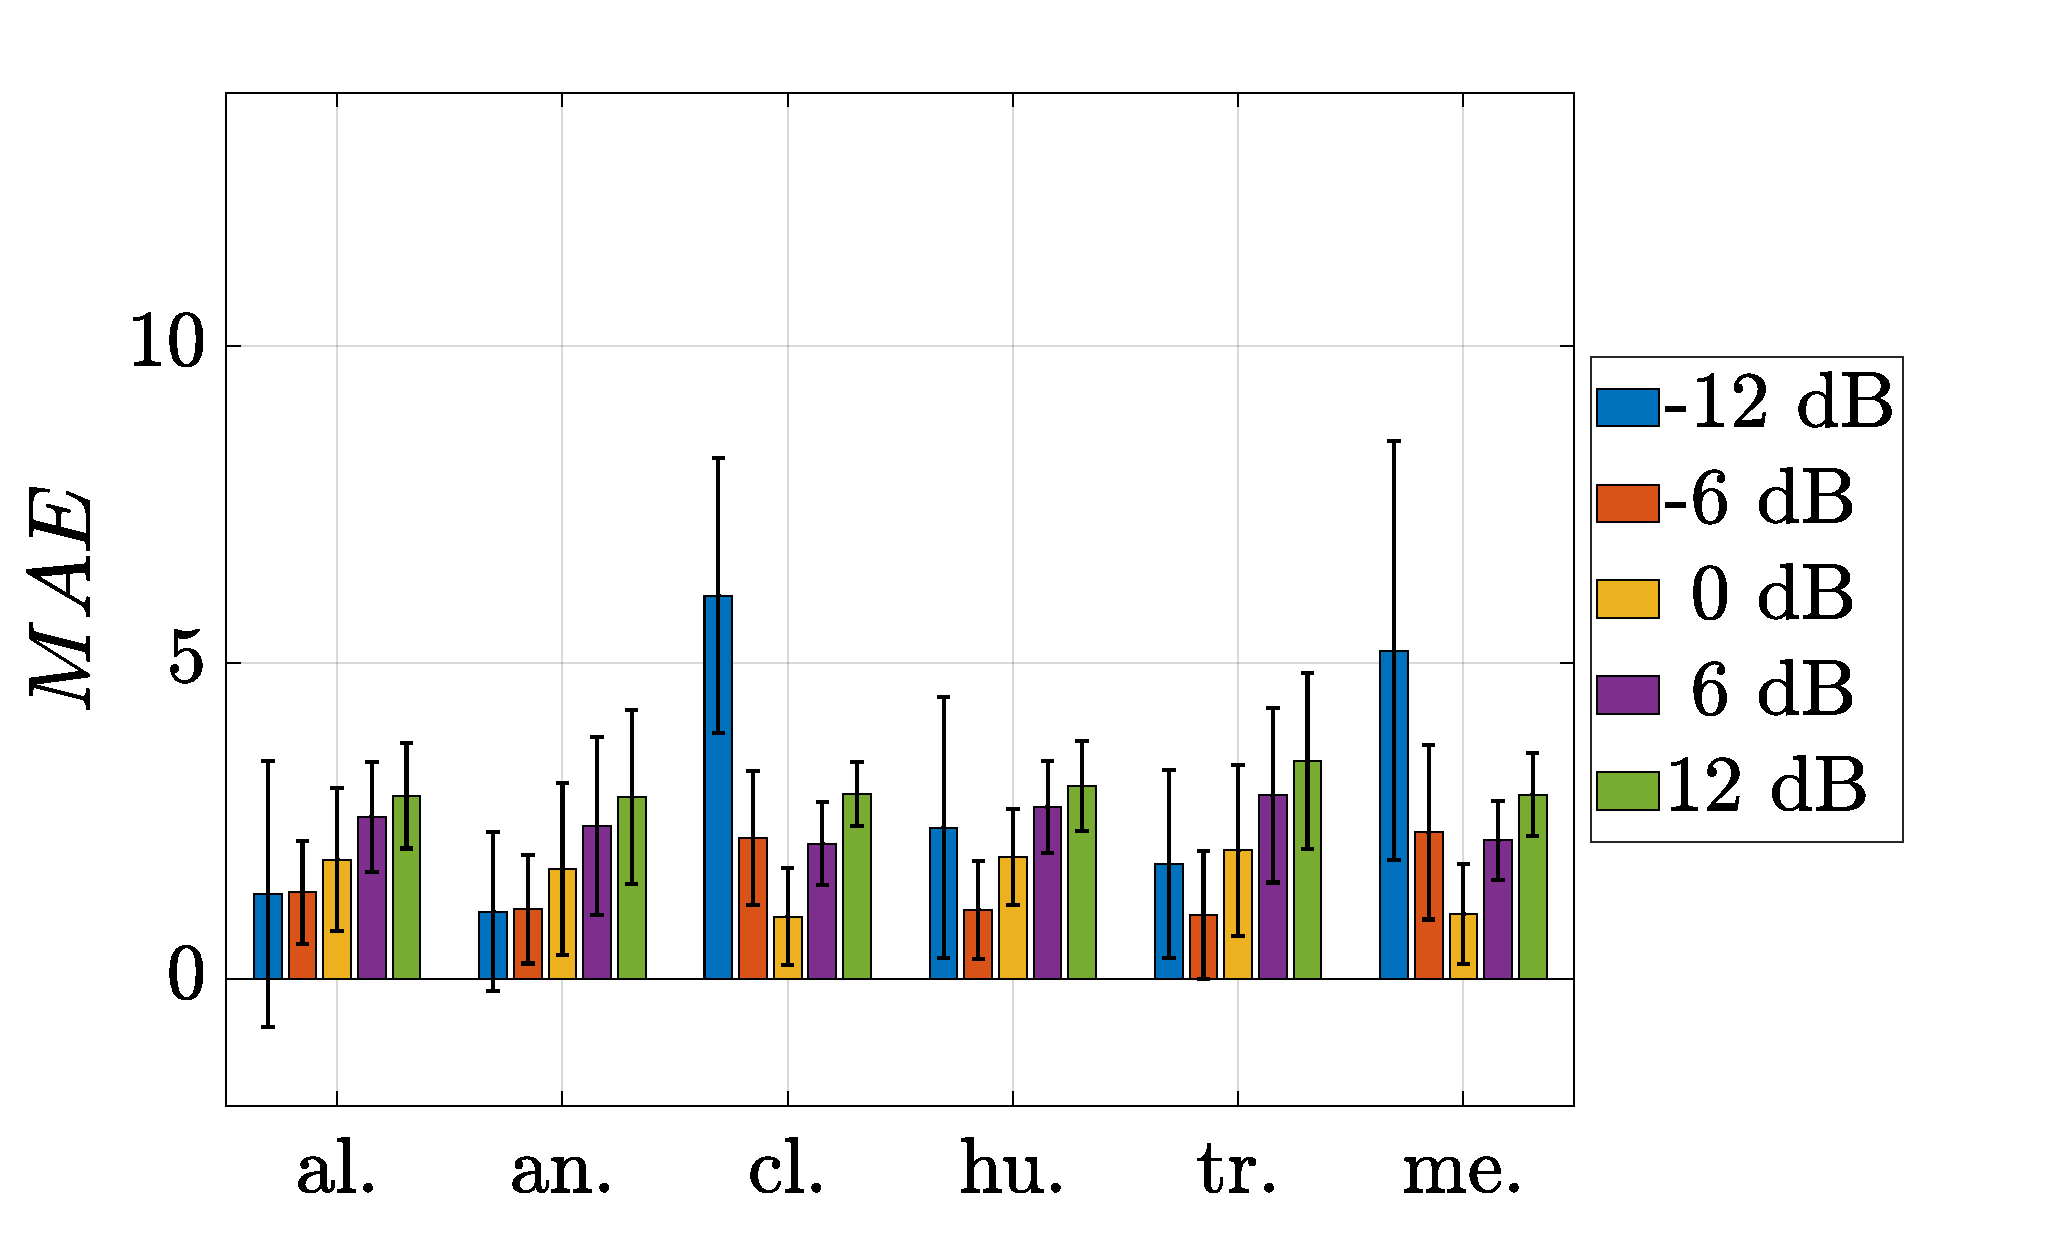
\includegraphics[width=0.60\linewidth]{./figures/resultats/ambiance_sem_bar.pdf}}%
\qquad
\subfigure[Erreurs $MAE$ pour la NMF IS.]{%
\label{fig:TIR_class_IS}%
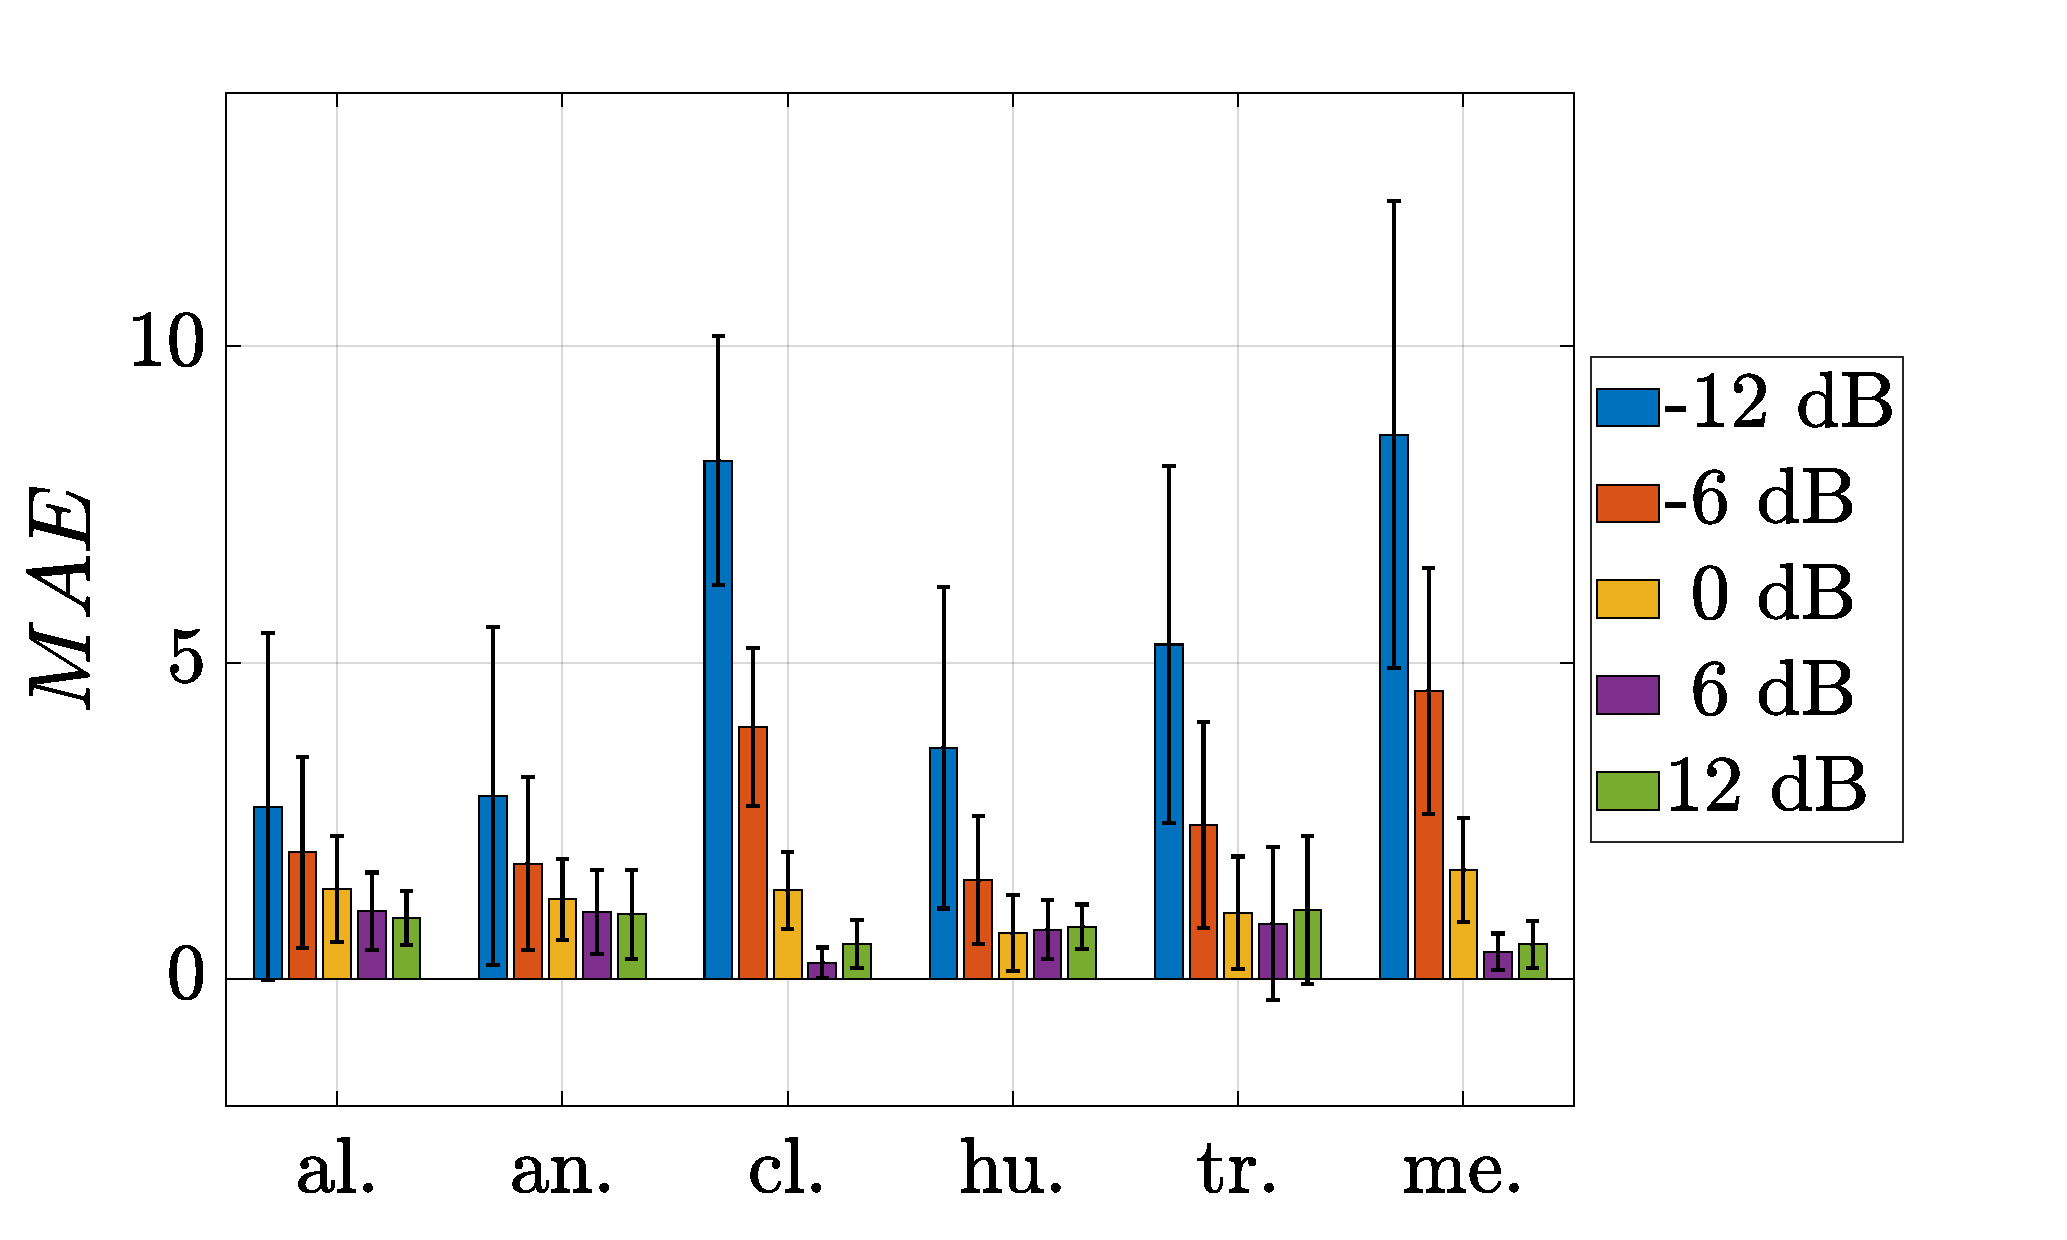
\includegraphics[width=0.60\linewidth]{./figures/resultats/ambiance_ti_bar.pdf}}%
\caption{Erreurs $MAE$ pour chaque classe pour la NMF SUP (\ref{fig:TIR_class_sup}), SEM (\ref{fig:TIR_class_semi}) et IS (\ref{fig:TIR_class_IS}).}
\end{figure}

Dans les Figures \ref{fig:TIR_bar}, les erreurs $MAE$ des 3 méthodes NMF optimales pour chaque $TIR$ et chaque ambiance sont résumés. La Figure \ref{fig:TIR_class_sup} permet de visualiser les performance très variable de la NMF SUP. Dans le cas où $TIR$ = $\lbrace -12, -6 \rbrace$ dB, et ceux pour les 6 cous-corpus, la NMF SUP obtient de fortes erreurs $MAE$. L'allure spectrale similaire à celle du trafic fit que ces erreurs sont élevé pour les sous-classes \textit{climat}, \textit{humains}, \textit{transport} et \textit{mécanique}. Même pour les sous-classes \textit{alerte} et \textit{animaux}, la méthode échoue a obtenir des faibles erreurs. Ces performances sont toutefois contre-balancé par les erreurs dans les hauts $TIR$ où les erreurs sont beacoup plus faibles, notamment à $TIR$ = 6 dB. La présence exclusive de trafic dans le dictionnaire où le trafic devient prédominant fonctionne, ici, correctement.

La NMF SEM (Figure \ref{fig:TIR_class_semi}), présente un comportement différent : les erreurs sont plus faibles lorsque le $TIR$ est négatif, hormis pour les sous-classes \textit{climat}  et \textit{mécanique}. L'ajout de $\mathbf{W_r}$ est donc déterminant. Cependant, lorsque le TIR devient positif et le trafic dominant, l'erreur augmente pour chaque sous-classe.
On compare dans les Figures \label{fig:Y_ambiance} les deux élements de $W_r$ obtenue pour une scène \textit{alerte} et \textit{climat} avec les spectres des signaux trafic et interférant à $TIR$ = $\lbrace -12, 12 \rbrace$ dB. Dans les cas où $TIR$ = -12 dB, la somme des éléments libres $\mathbf{W_r}$ correspond bien au spectre de la classe \textit{interférante}. Ces deux éléments permettent donc bien de modéliser cette classe, laissant la partie \textit{trafic} au dictionnaire $\mathbf{W_s}$. À l'opposée, pour $TIR$ = 12 dB, l'allure de $\mathbf{W_r}$ ne suit plus la celle de la classe \textit{interférante}. Certaines parties des spectres modélisent participent alors à la modélisation de la composante \textit{trafic}, ce qui réduit la justesse de son estimation du niveau sonore. Les degrés de liberté de la NMF SEM sont donc un avantage lorsque le trafic est peu présent car ils permettent bien d'intégrer la classe de son interférante. Mais cette liberté joue en sa défaveur lors que celui-ci devient prédominant où des composantes \textit{trafic} sont inclus.\\

\begin{figure}%
\centering
\subfigure[Comparaison pour $TIR$ = -12 dB pour la scène 2 du sous-corpus \textit{alerte}.]{%
\label{fig:Y_alert_-12}%
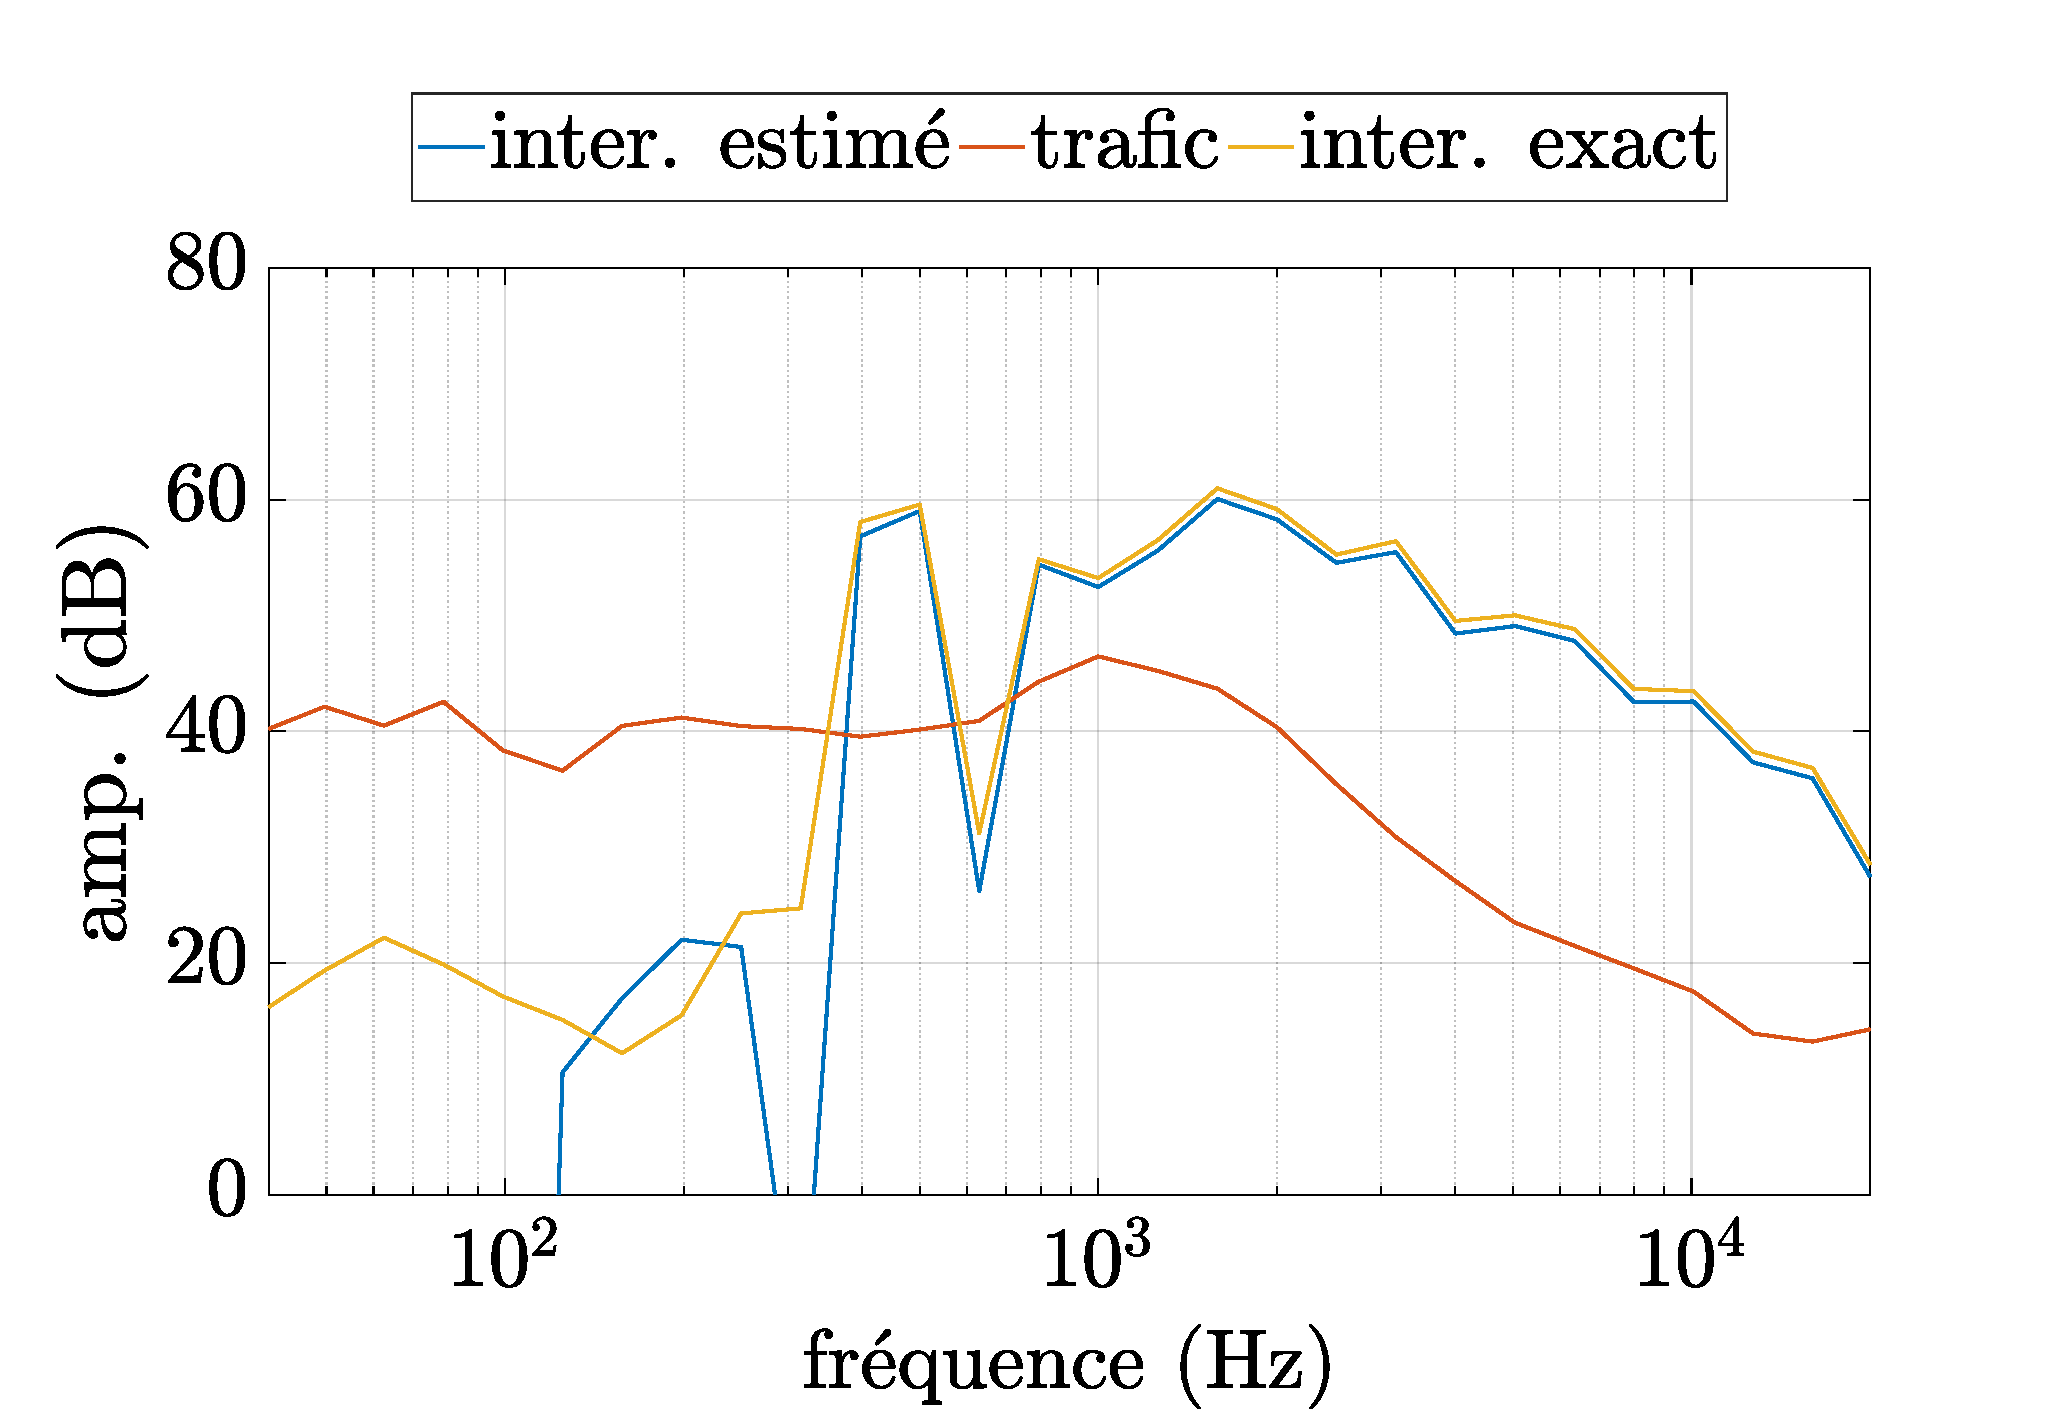
\includegraphics[width=0.450\linewidth]{./figures/resultats/alert02_tir-12_Y.pdf}}%
\qquad
\subfigure[Comparaison pour $TIR$ = 12 dB pour la scène 2 du sous-corpus \textit{alerte}.]{%
\label{fig:Y_alert_12}%
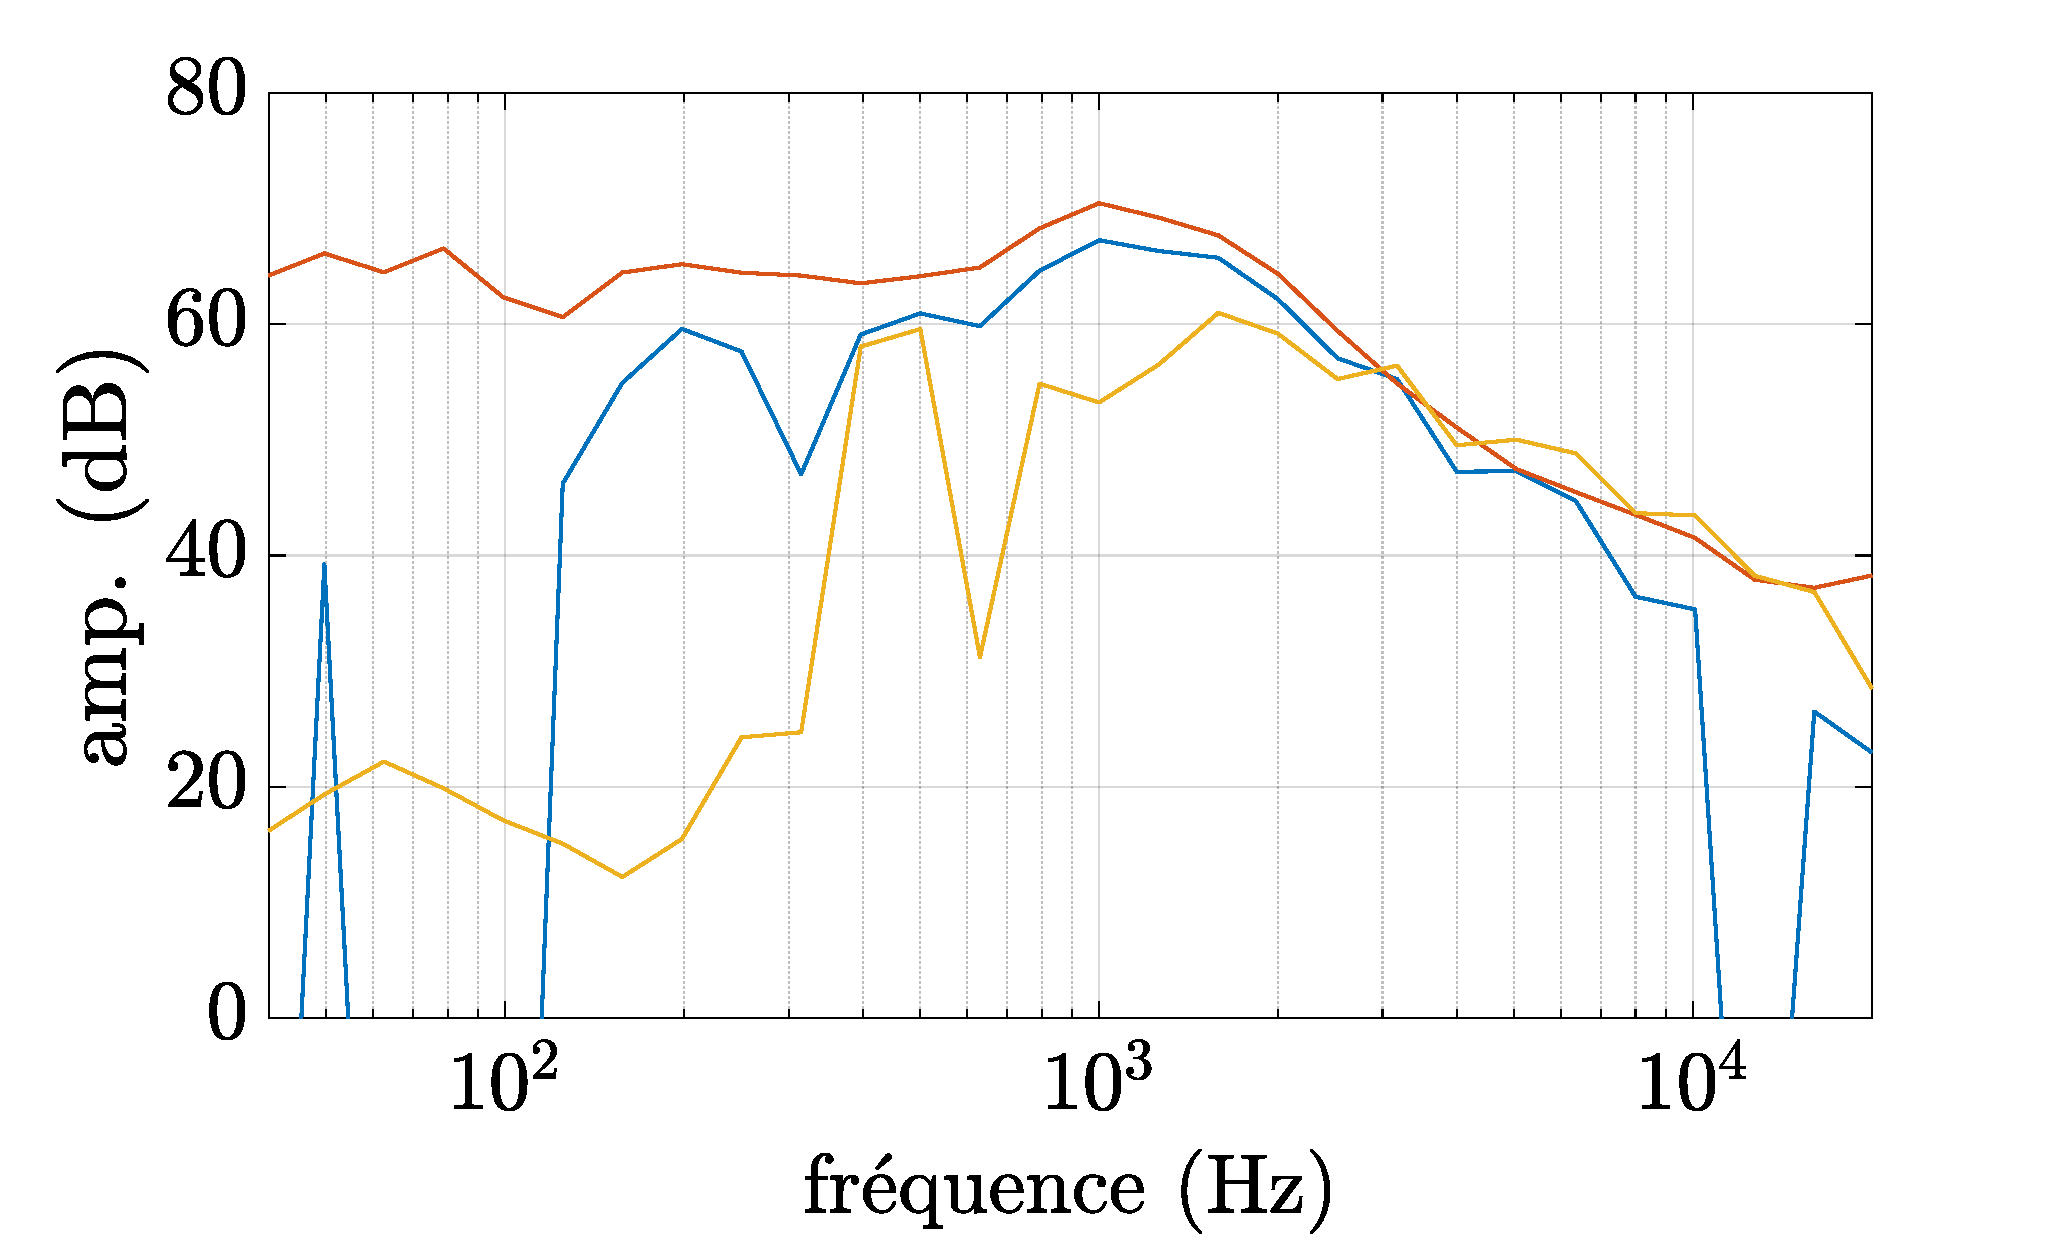
\includegraphics[width=0.450\linewidth]{./figures/resultats/alert02_tir12_Y.pdf}}%
\qquad
\subfigure[Comparaison pour $TIR$ = -12 dB pour la scène 3 du sous-corpus \textit{climat}.]{%
\label{fig:Y_climat_-12}%
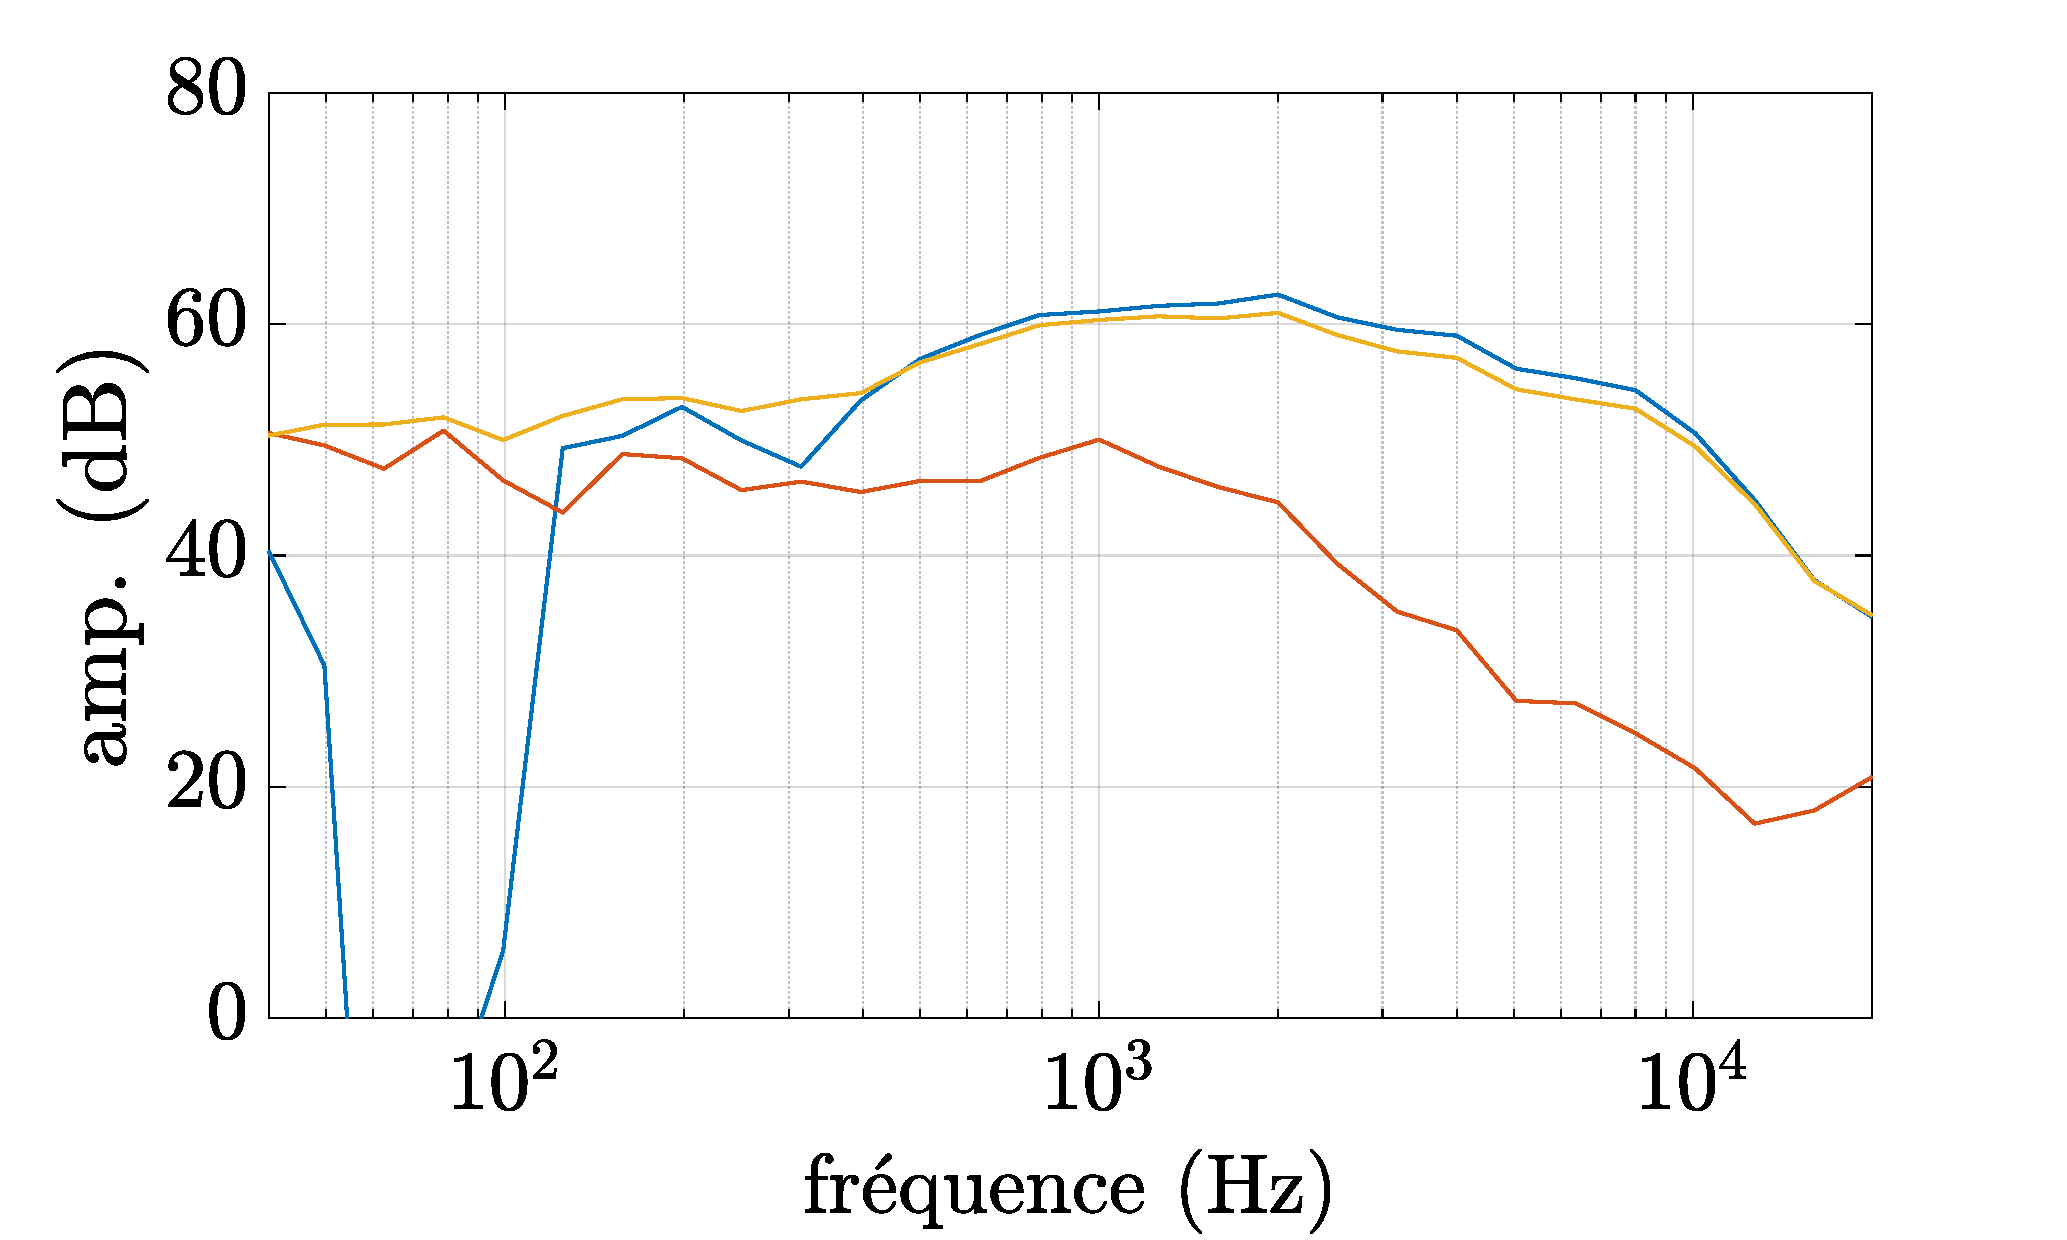
\includegraphics[width=0.450\linewidth]{./figures/resultats/climat03_tir-12_Y.pdf}}%
\qquad
\subfigure[Comparaison pour $TIR$ = 12 dB pour la scène 3 du sous-corpus \textit{climat}.]{%
\label{fig:Y_climat_12}%
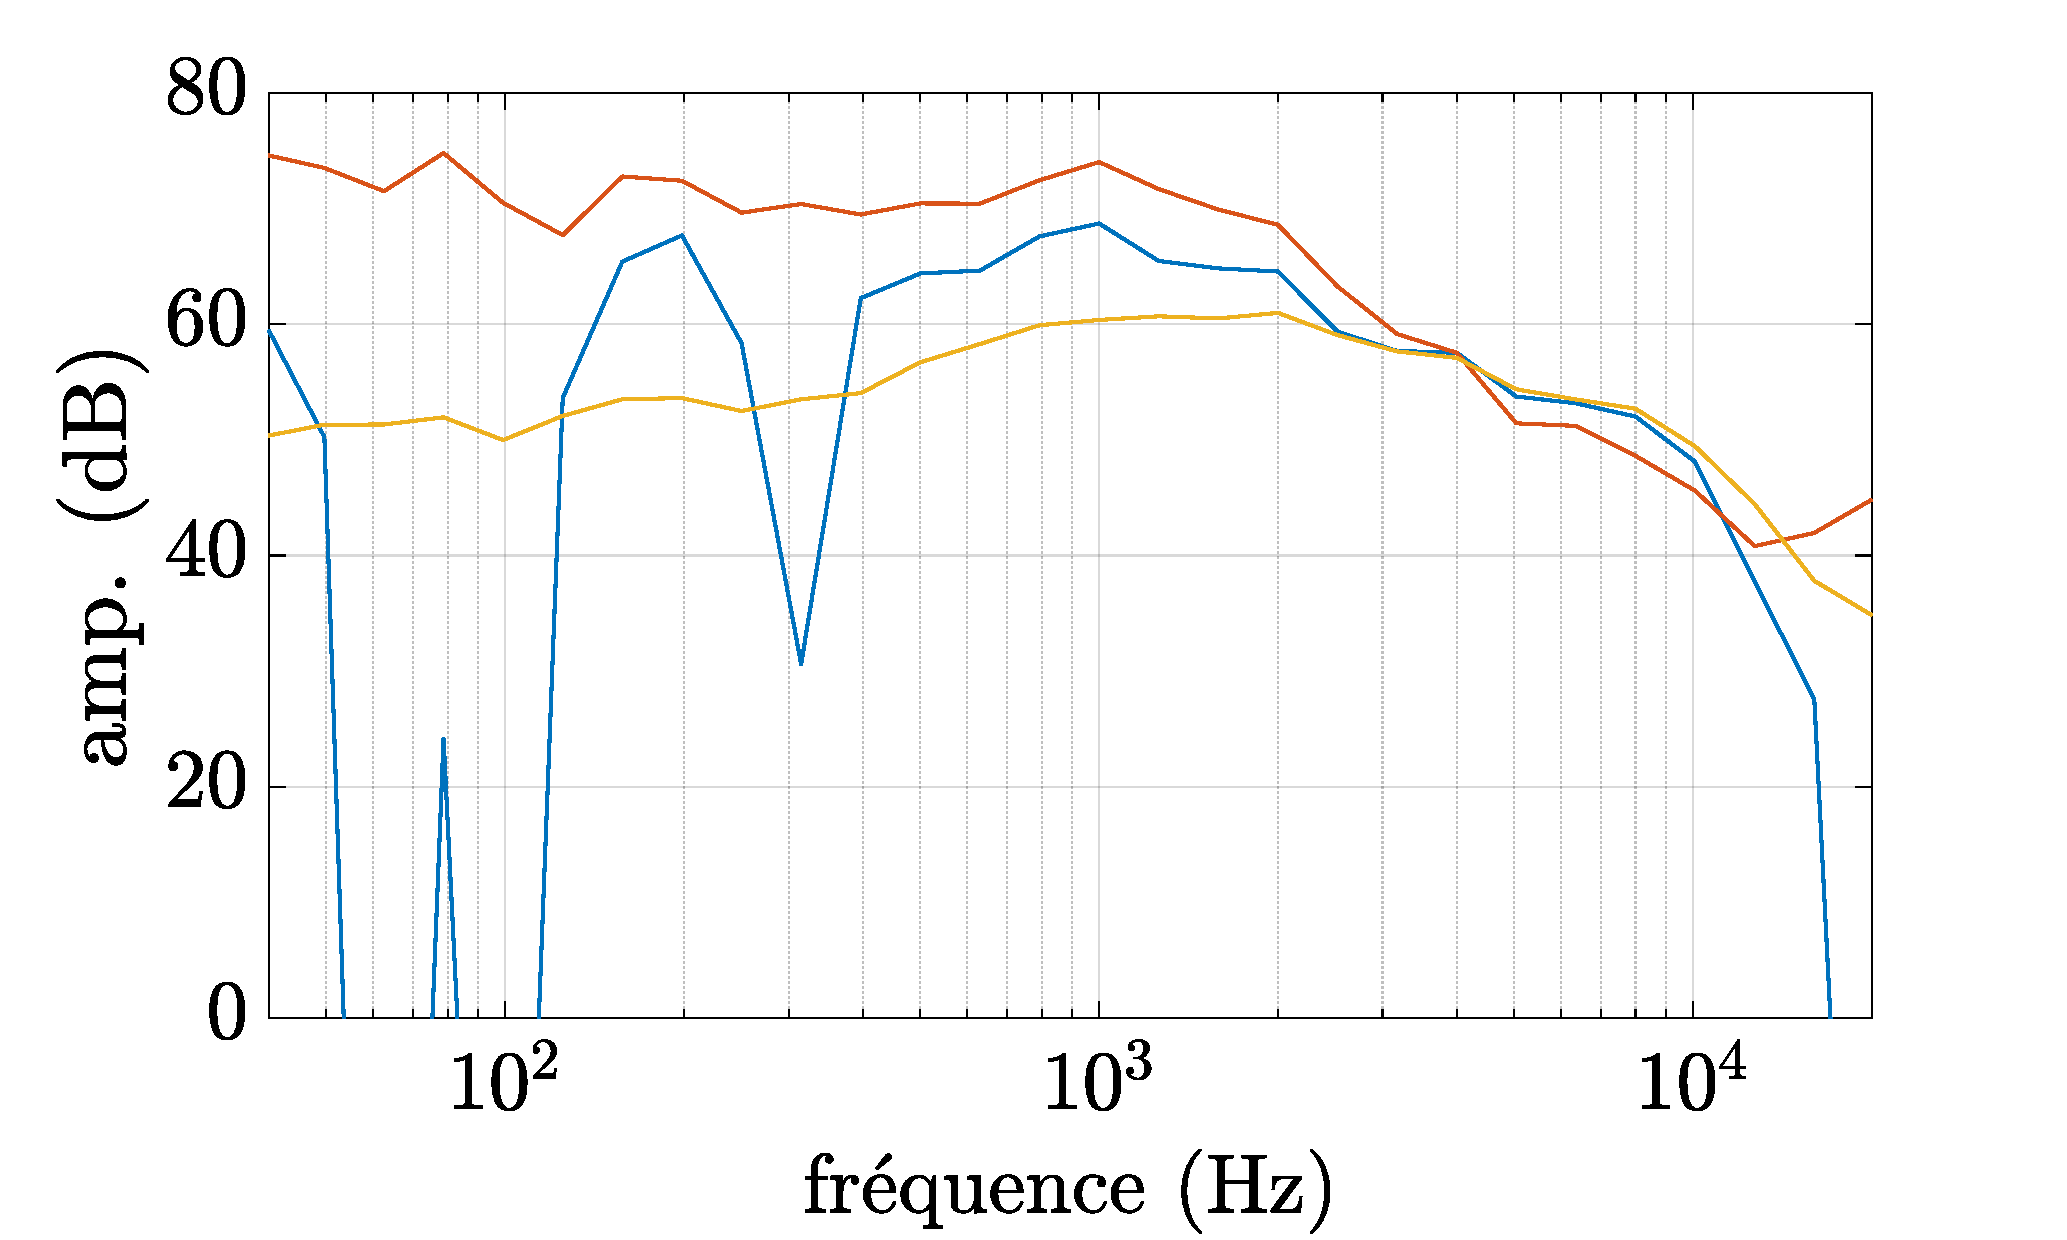
\includegraphics[width=0.450\linewidth]{./figures/resultats/climat03_tir12_Y.pdf}}%
\caption{Comparaisons des spectres des classes \textit{trafic} et \textit{interférante} avec la somme des 2 éléments de $\mathbf{W_r}$ pour 2 valeurs du $TIR$ (-12 dB et 12 dB) pour 2 sous-corpus (\textit{alerte} et \textit{climat)}}
\label{fig:Y_ambiance}
\end{figure}

Enfin, la NMF IS présente une allure similaire à celle de la NMF SUP (erreur plus forte au faible TIR pour être plus petite dans les haut TIR), mais avec des valeurs d'erreurs bien plus faibles. La méthode améliore significativement les erreurs pour les TIR négatifs. Toutefois les erreurs pour les sous-classes \textit{climat}, \textit{transport} et \textit{mécanique} restent élevées en raison de la proximité de leur spectre avec ceux du trafic. Pour $TIR \geq 0$, les erreurs restent faibles ($< 1,7$ dB). La mise à jours du dictionnaire permet de mieux ajuster $\mathbf{W}$ à la scène et ainsi à la source trafic. Toutefois, lorsque le TIR est négatif, en choisissant un seuil fixe sur l'ensemble du corpus, celui-ci est susceptible d'être trop élevé et d'intégrer des éléments qui ne sont pas \textit{trafic} dans $\mathbf{W_{trafic}}$. 
La valeur seuil de 0,41 est la valeur optimale permettant une erreur minimale sur l'intégralité du corpus, mais selon le sous-corpus ou le $TIR$ ce seuil optimale peut varier. Dans les Figures \ref{TIR_mae}, l'évolution du TIR est tracé en fonction du seuil $t_h$ et du sous-corpus. Selon la classe de son
Pour $TIR$ = -12 dB, l'erreur $MAE$ minimale diffèrent selon les sous-corpus. Dans le cas du \textit{climat} et de \textit{mécanique}, le seuil $t_h$ est même élevé. Ainsi, pour les classes de sons dont l'allure spectrale est similaire à celle du trafic, le seuil optimale $t_h$ = 0,41 est un seuil pas assez élevé. Celui-ci gagnerait à être augmenté pour ainsi garder moins d'éléments susceptibles d'appartenir à la classe de sons interférante dans le dictionnaire.
Ainsi, la valeur seuil optimale pour $TIR$ = -12 dB est $t_h = 0,49$, sur l'ensemble des sous-corpus pour une erreur $MAE_{-12}$ = 4,61 ($\pm$ 1,91) avec un nombre moyen d'éléments $K$ = 79 ($\pm$ 22). 
À l'inverse, pour des TIR élevés, l'ensemble des sous-corpus trouve une erreur $MAE$ minimale pour un seuil faible. Le trafic devenant prédominant, le dictionnaire $\mathbf{W'}$ mis à jours contient plus d'éléments trafic. En diminuant le seuil $t_h$ il est possible d'intégrer plus d'éléments dans $\mathbf{W'}$. Il convient de ne pas le prendre trop bas afin de ne pas considérer des éléments de la classe interférante. Ainsi à partir de $t_h$ = 0,31 pour $TIR$ = 12 dB, un plus grand nombre d'élément du dictionnaire est considéré ($K_{moyen}$ = 142 ($\pm$ 22) et l'erreur $MAE_{+12}$ diminue à 0,20 ($\pm$ 0,08), soit une erreur inférieure au filtre passe-bas à 20 kHz.


\begin{figure}%
\centering
\subfigure[]{%
\label{fig:TIR_mae_tir-12}%
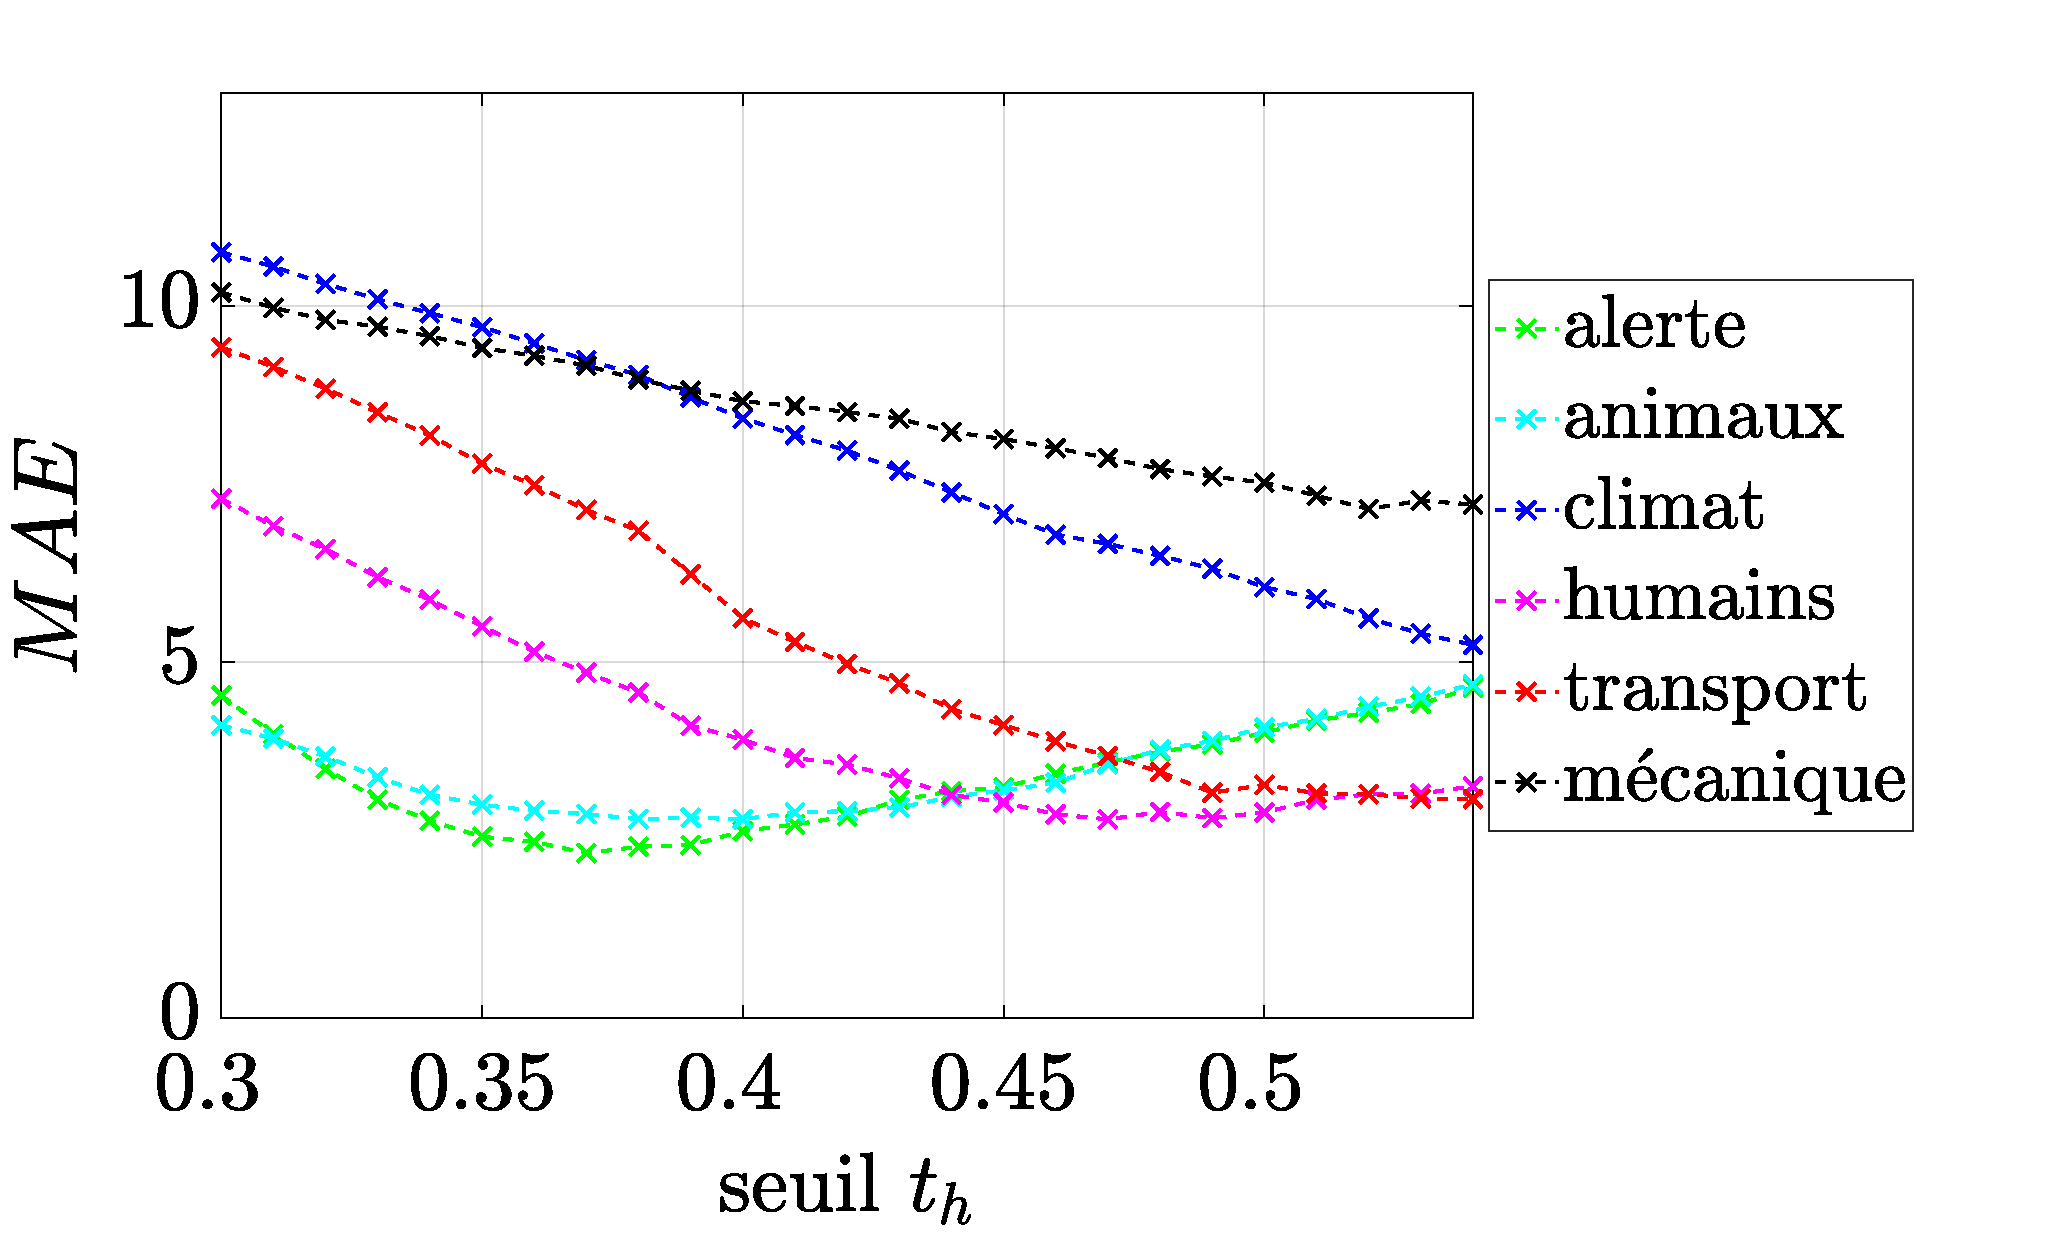
\includegraphics[width=0.60\linewidth]{./figures/resultats/ambiance_maeExpand_tir-12.pdf}}%
\qquad
\subfigure[]{%
\label{fig:TIR_mae_tir0}%
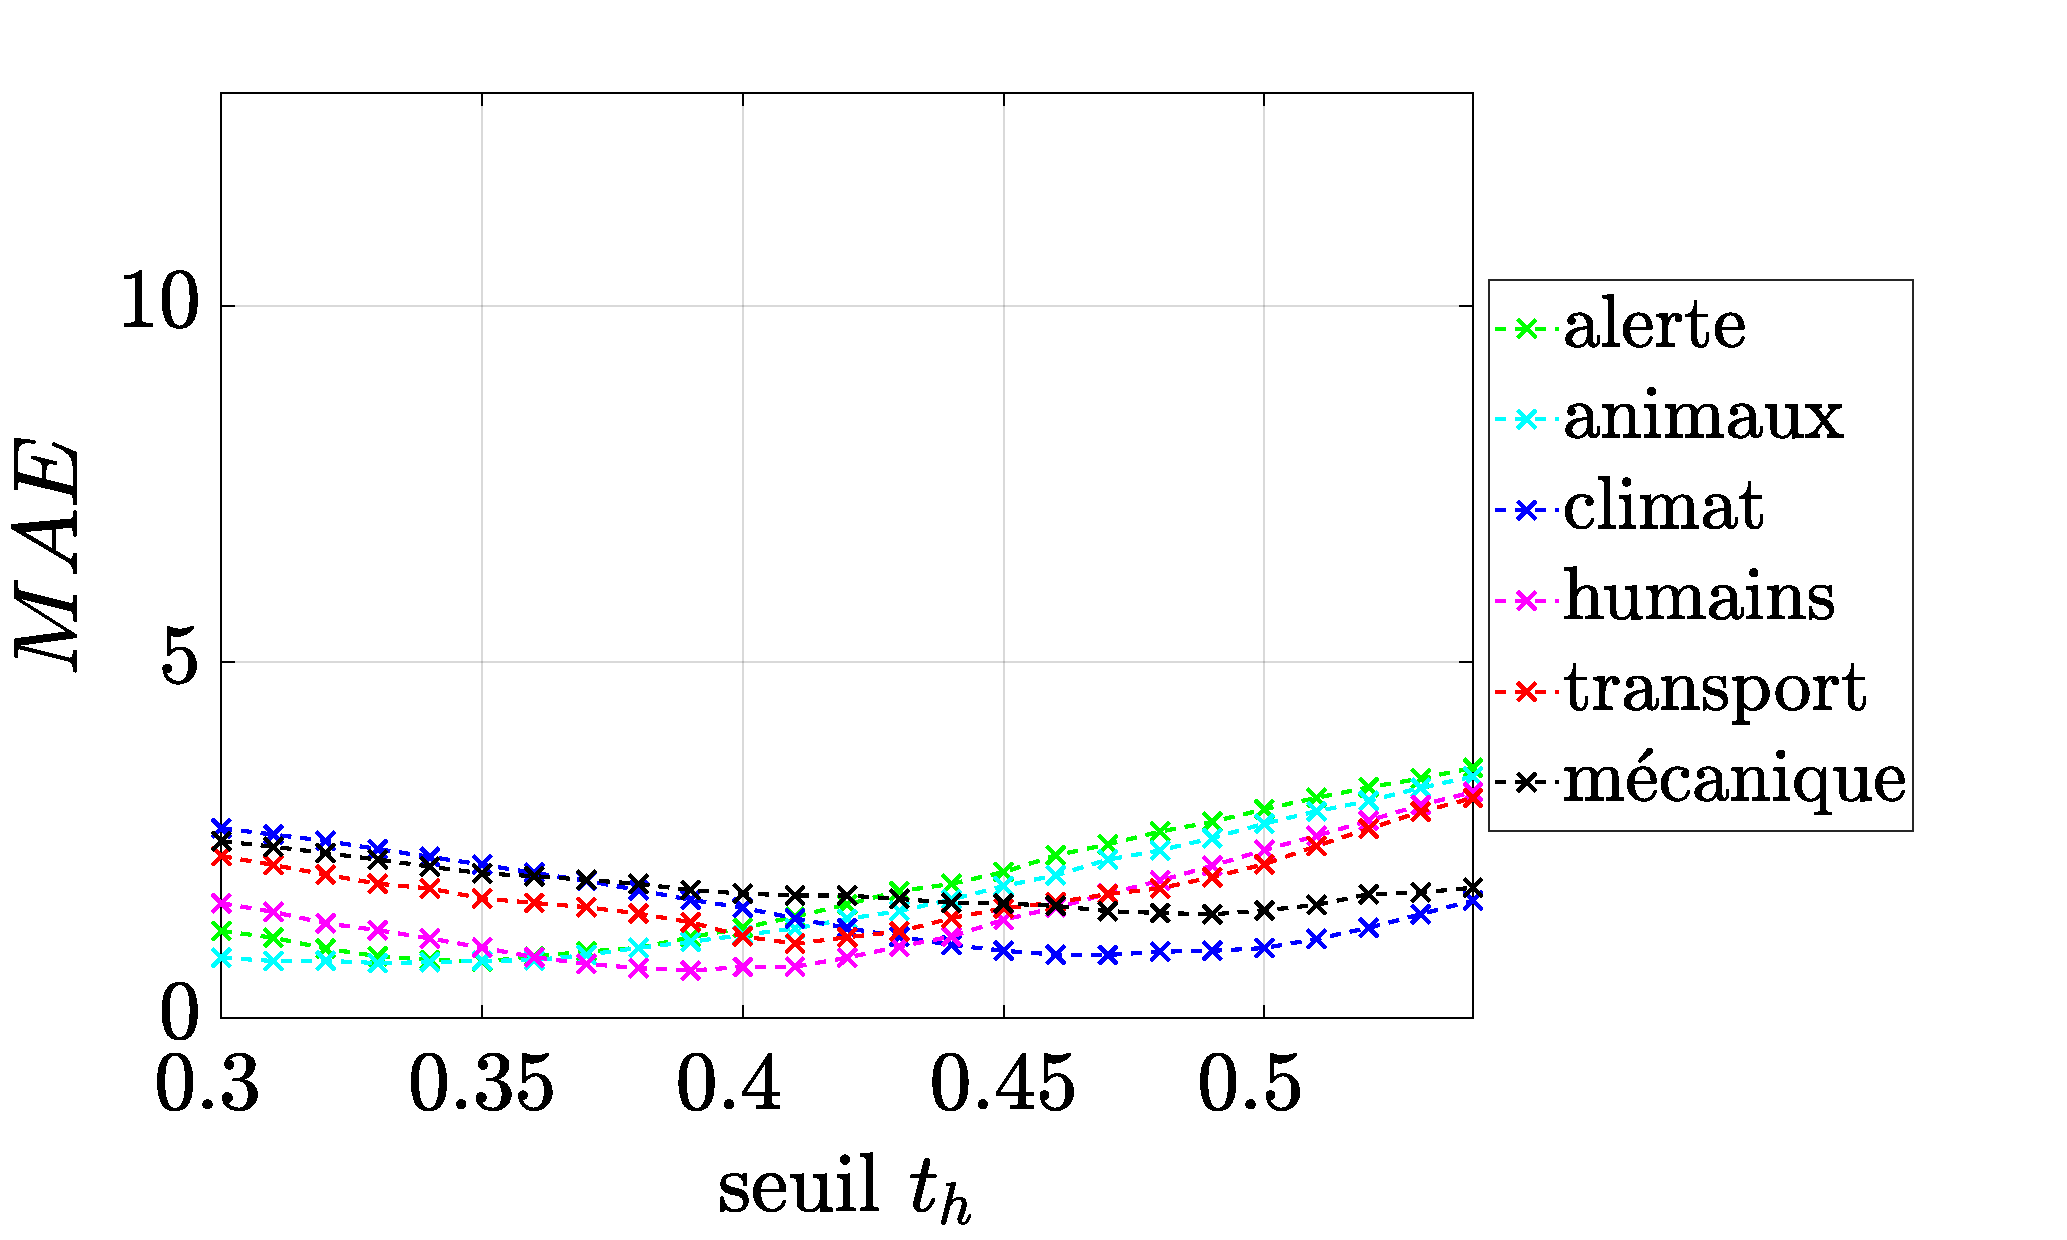
\includegraphics[width=0.60\linewidth]{./figures/resultats/ambiance_maeExpand_tir0.pdf}}%
\qquad
\subfigure[]{%
\label{fig:TIR_mae_tir12}%
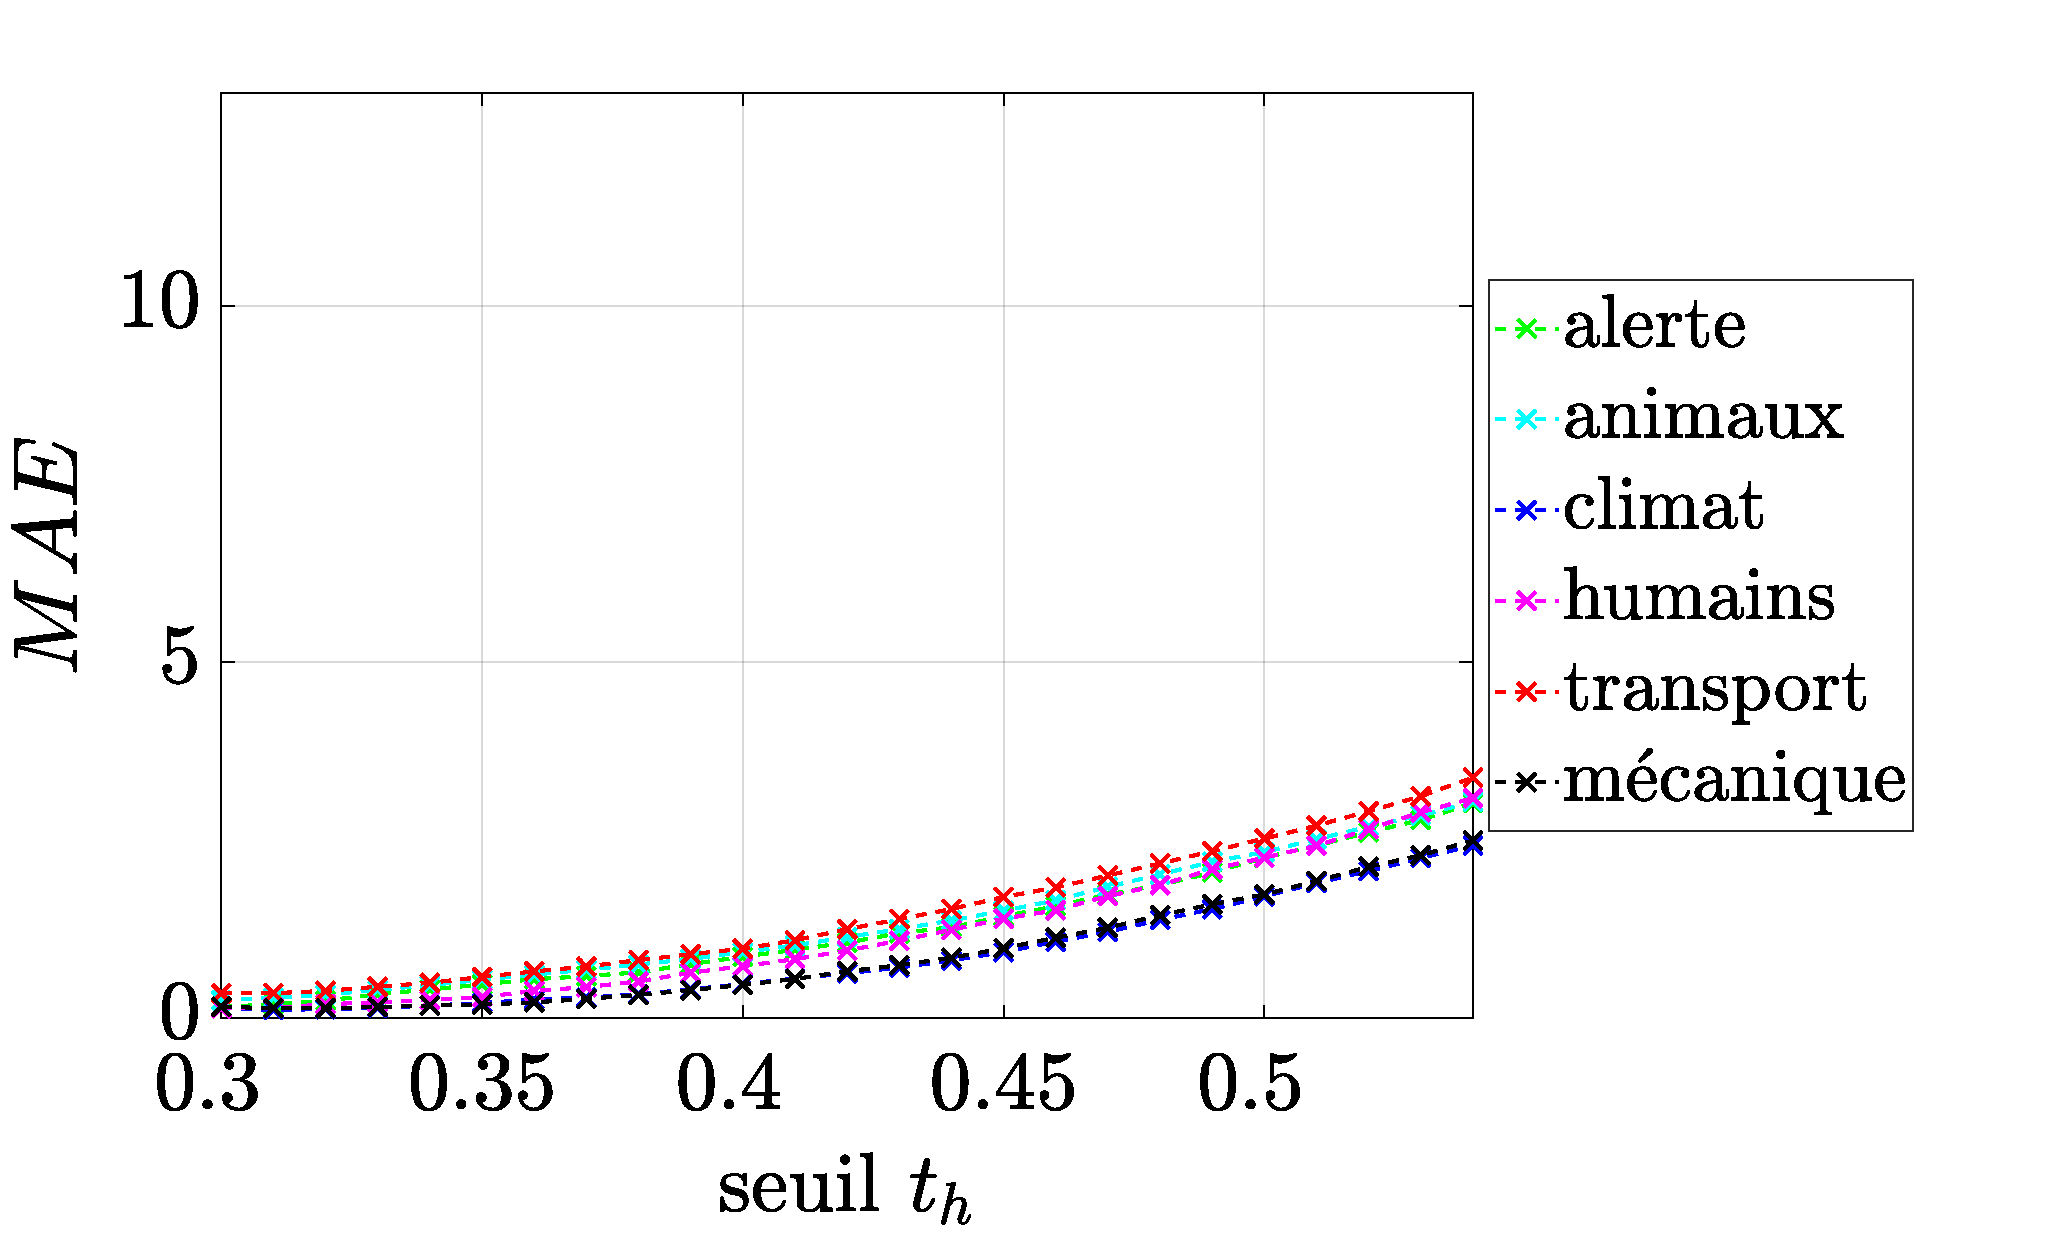
\includegraphics[width=0.60\linewidth]{./figures/resultats/ambiance_maeExpand_tir12.pdf}}%
\caption{Évolution de l'erreur $MAE$ pour chaque sous-corpus selon la valeur seuil $t_h$ pour $TIR = -12$ dB (\ref{fig:TIR_mae_tir-12}), $TIR = 0$ dB (\ref{fig:TIR_mae_tir0}) et $TIR = 12$ dB (\ref{fig:TIR_mae_tir12}).}
\label{fig:TIR_mae}
\end{figure}

\subsubsection{Convergence et temps de calcul}
Enfin, la fonction de coût $D(\mathbf{V}\Vert \mathbf{WH})$ est observé selon chaque TIR pour les 3 versions de la NMF.

Pour chaque NMF, la convergence des algorithmes est plus rapide pour les $TIR$ négatif que les $TIR$ positifs. Le NMF SEM est celle dont la fonction coût est la plus importante. 
Pour la NMF SUP, les valeurs de la fonction de coût sont faibles et convergent vite dans le cas ou $TIR < 0$ dB. Ce phénomène traduit bien ces mauvaises performances : l'algorithme tente de reconstruire l'intégralité du signal avec les éléments qu'il possède dans le dictionnaire. Se faisant, les éléments trafic sont alors utilisés afin de modéliser la classe de son interférante. Pour la NMF IS, la fonction coût est initialement élevé pour rapidement converger vers une solution nulle. Ici, cette convergence est aidée par la mise à jours de la matrice $\mathbf{W}$. 

\begin{figure}[hbtp]
\centering
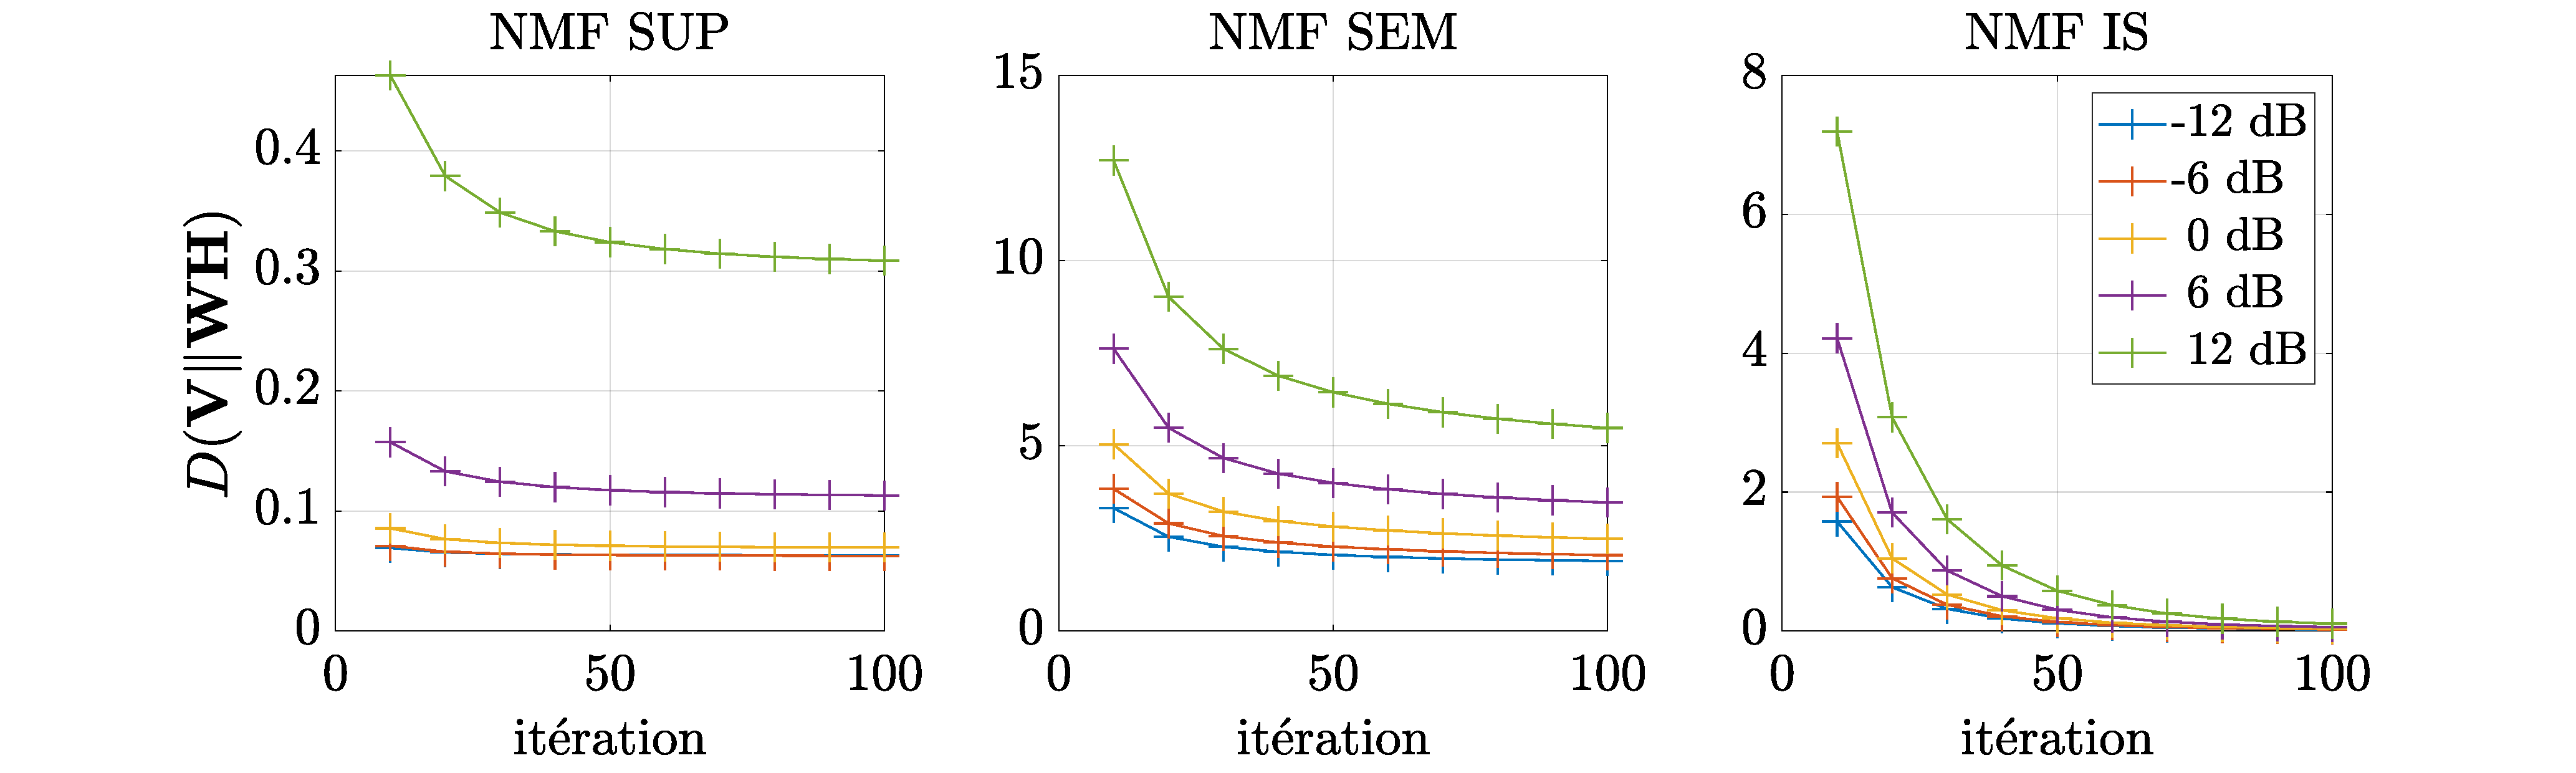
\includegraphics[width=.8\linewidth]{./figures/resultats/ambiance_cost.pdf}
\caption{Fonction de coût moyenné sur les sous-coprus pour chaque TIR et chaque version de la NMF}
\end{figure}


%\end{document}
